\subsection{User Interfaces}

\begin{center}
	\textbf{Third Party's Web Interface}
\end{center}

\begin{figure}[H]
    \centering
    \frame{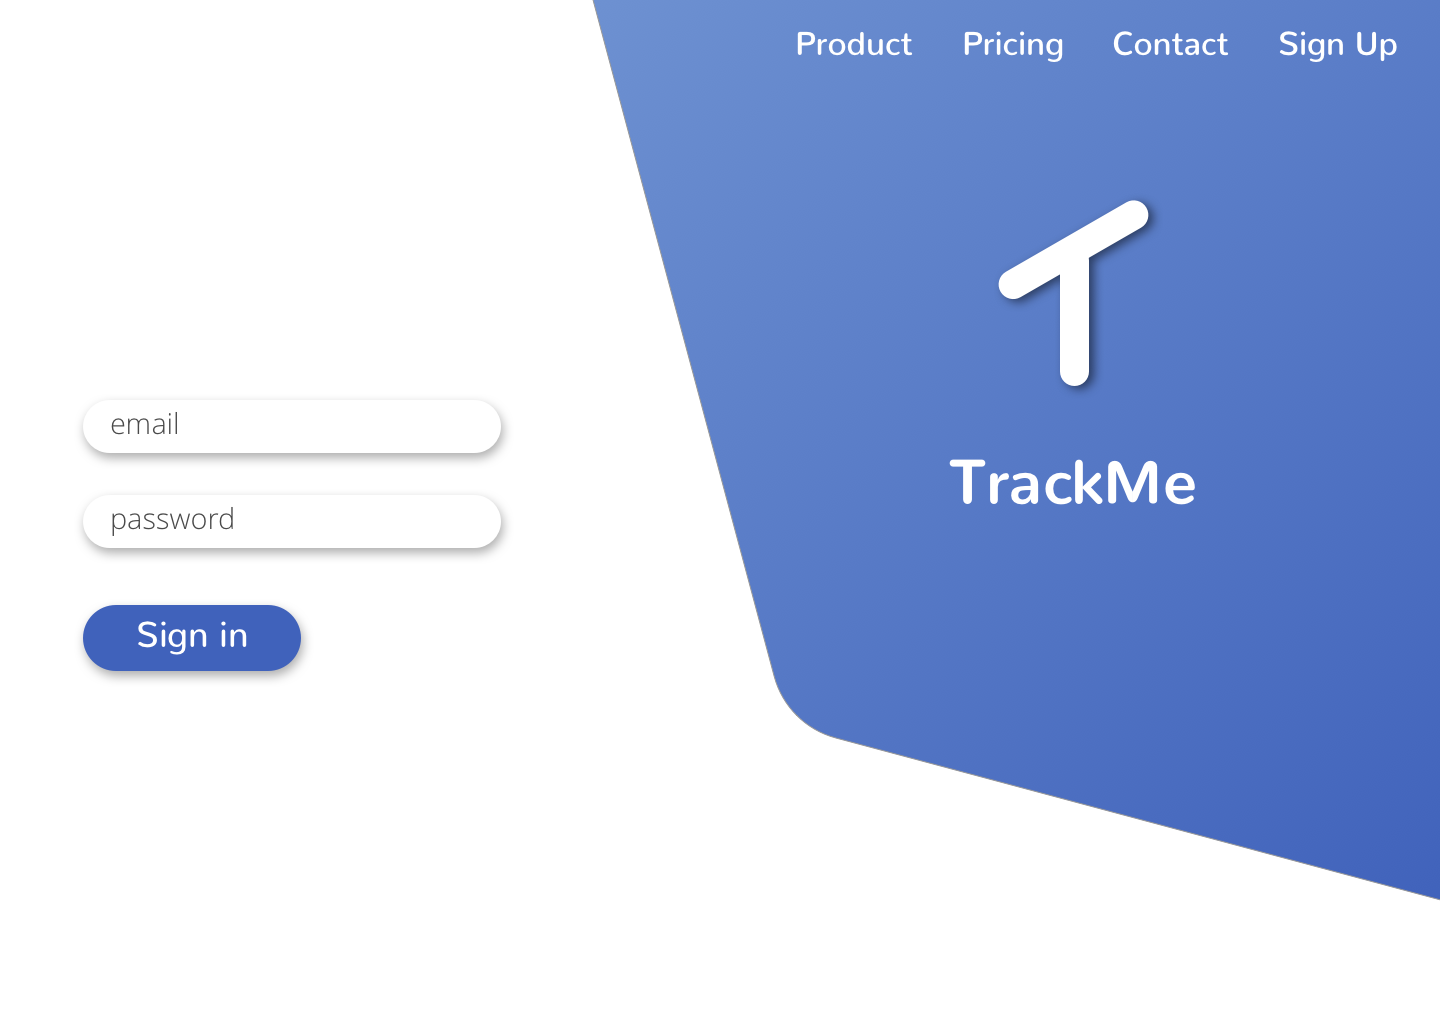
\includegraphics[scale=0.27]{./Pictures/Mockup/web/login.png}}
    \caption{Log-in on the web application of  \emph{TrackMe} System}
\end{figure}

\begin{figure}[H]
    \centering
    \frame{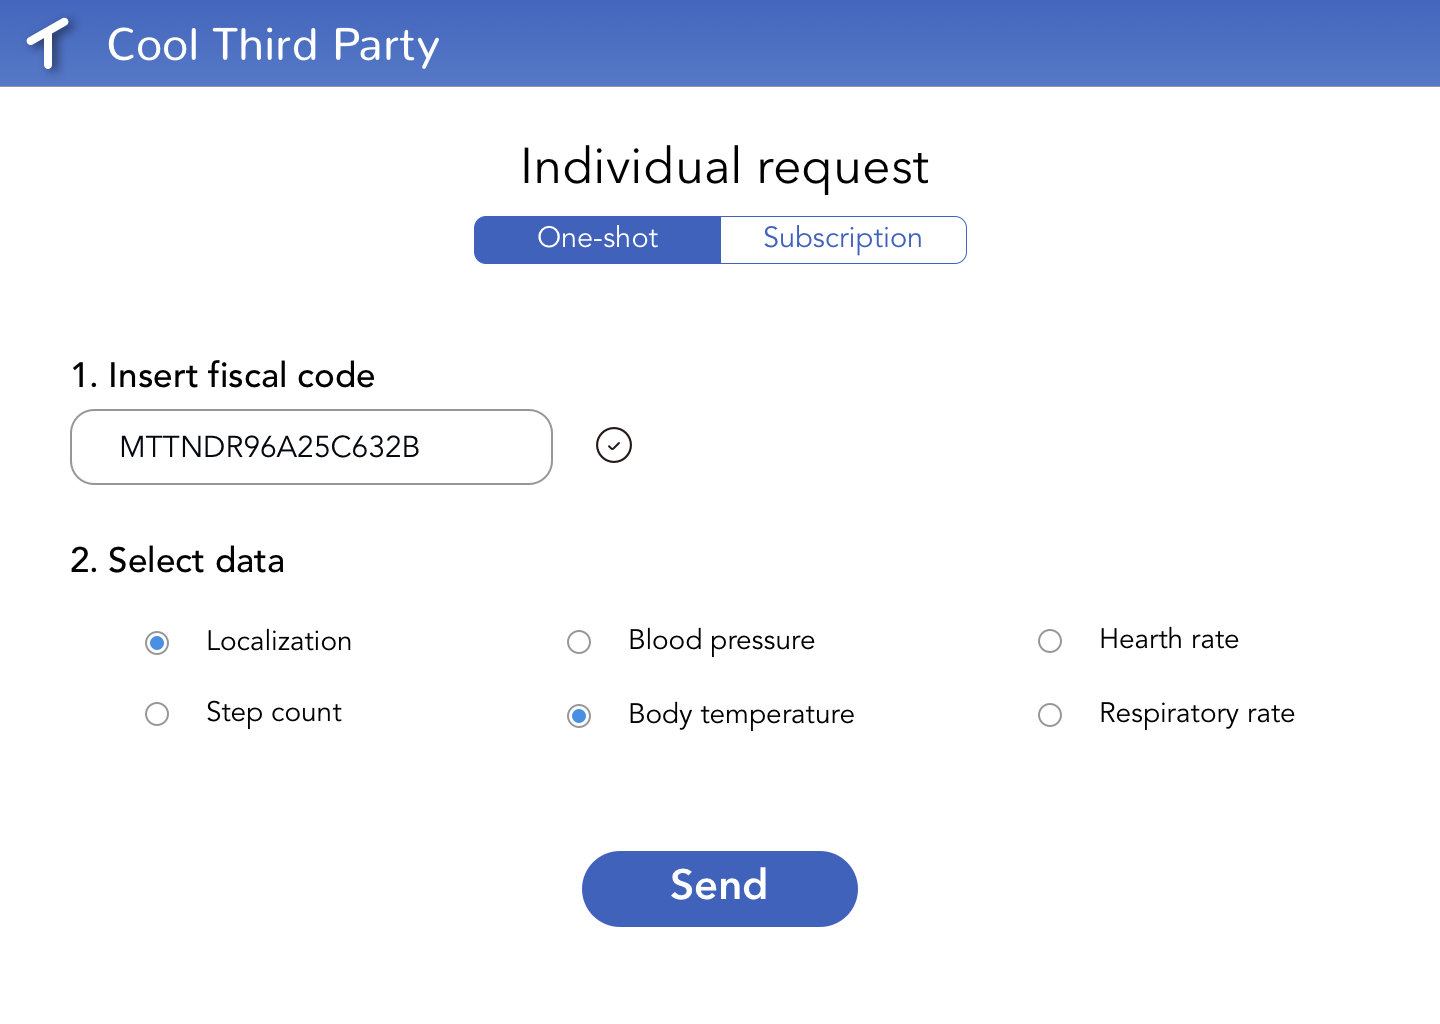
\includegraphics[scale=0.27]{./Pictures/Mockup/web/individual1.png}}
    \caption{One-shot user request}
\end{figure}

\begin{figure}[H]
    \centering
    \frame{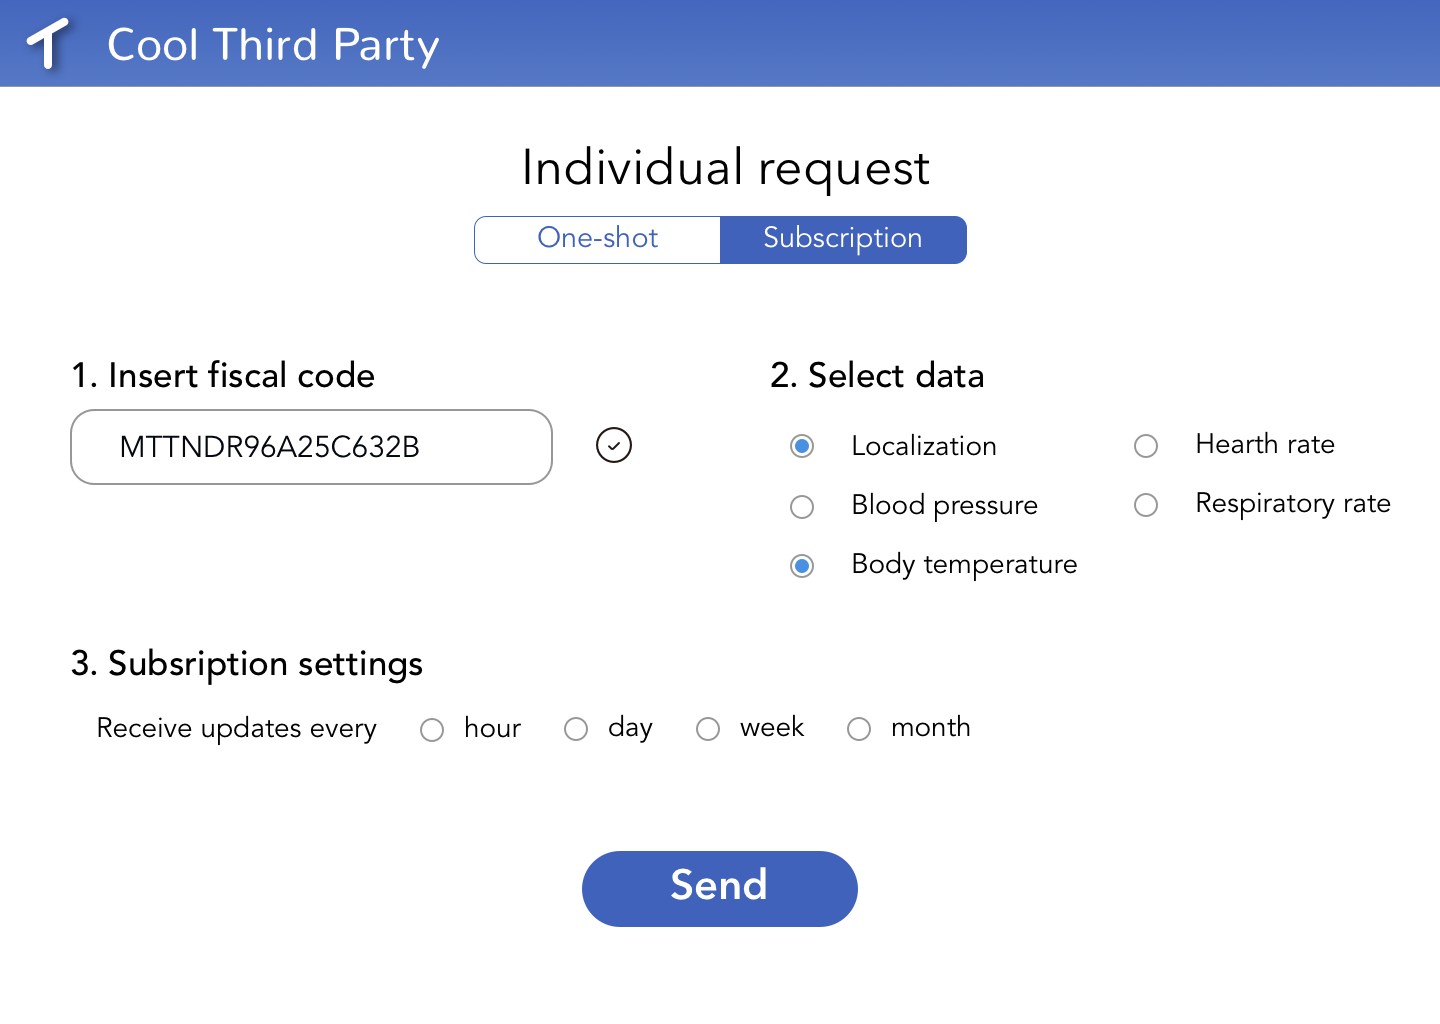
\includegraphics[scale=0.27]{./Pictures/Mockup/web/individual2.png}}
    \caption{Subscription user request}
\end{figure}

\begin{figure}[H]
    \centering
    \frame{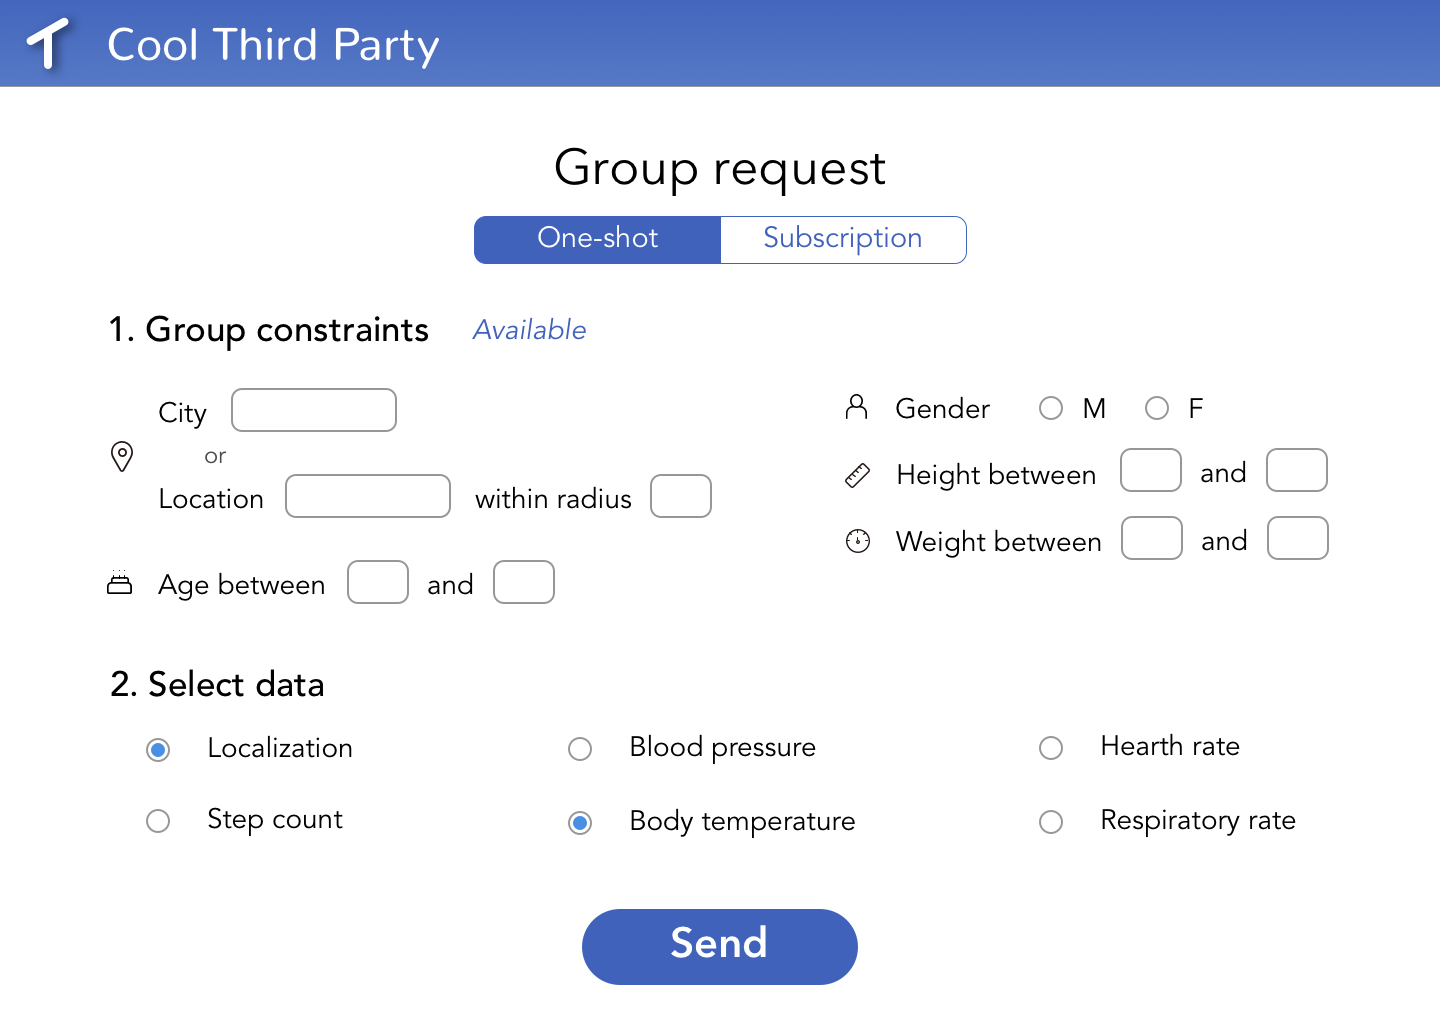
\includegraphics[scale=0.27]{./Pictures/Mockup/web/group1.png}}
    \caption{One-shot group request}
\end{figure}

\begin{figure}[H]
    \centering
    \frame{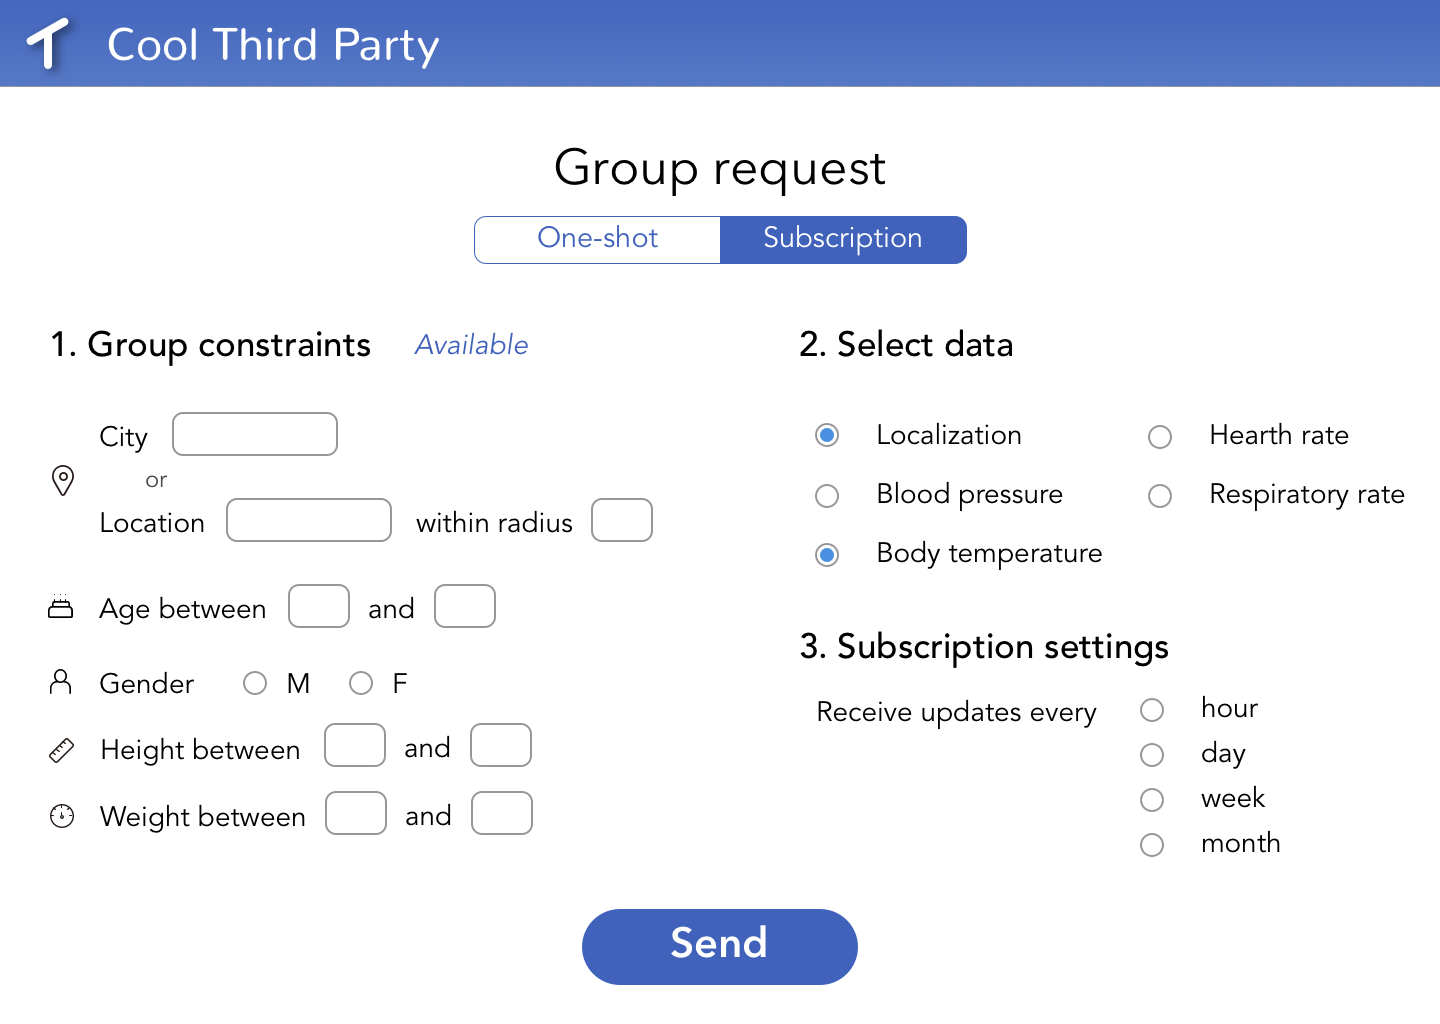
\includegraphics[scale=0.27]{./Pictures/Mockup/web/group2.png}}
    \caption{Subscription group request}
\end{figure}

\begin{figure}[H]
    \centering
    \frame{\includegraphics[scale=0.27]{./Pictures/Mockup/web/individuals-data.png}}
    \caption{Performed Requests}
\end{figure}

\begin{figure}[H]
    \centering
    \frame{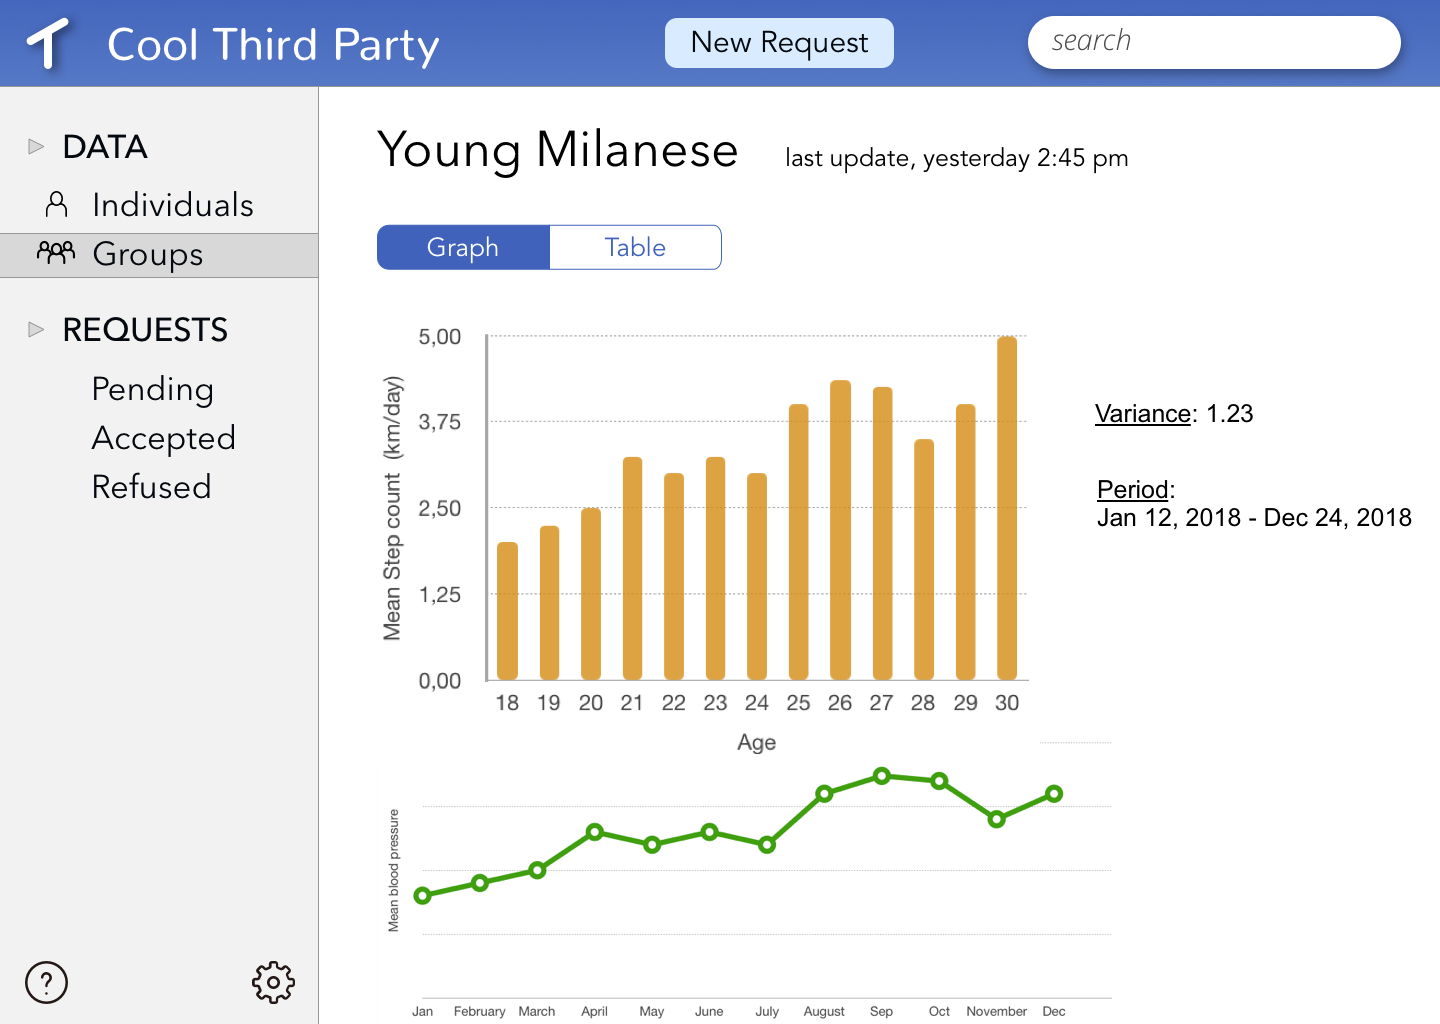
\includegraphics[scale=0.27]{./Pictures/Mockup/web/stats.png}}
    \caption{Results of a group request }
\end{figure}



\newpage


\begin{center}
	\textbf{User's Mobile Interface}
\end{center}

\begin{figure}[H]
    \centering
    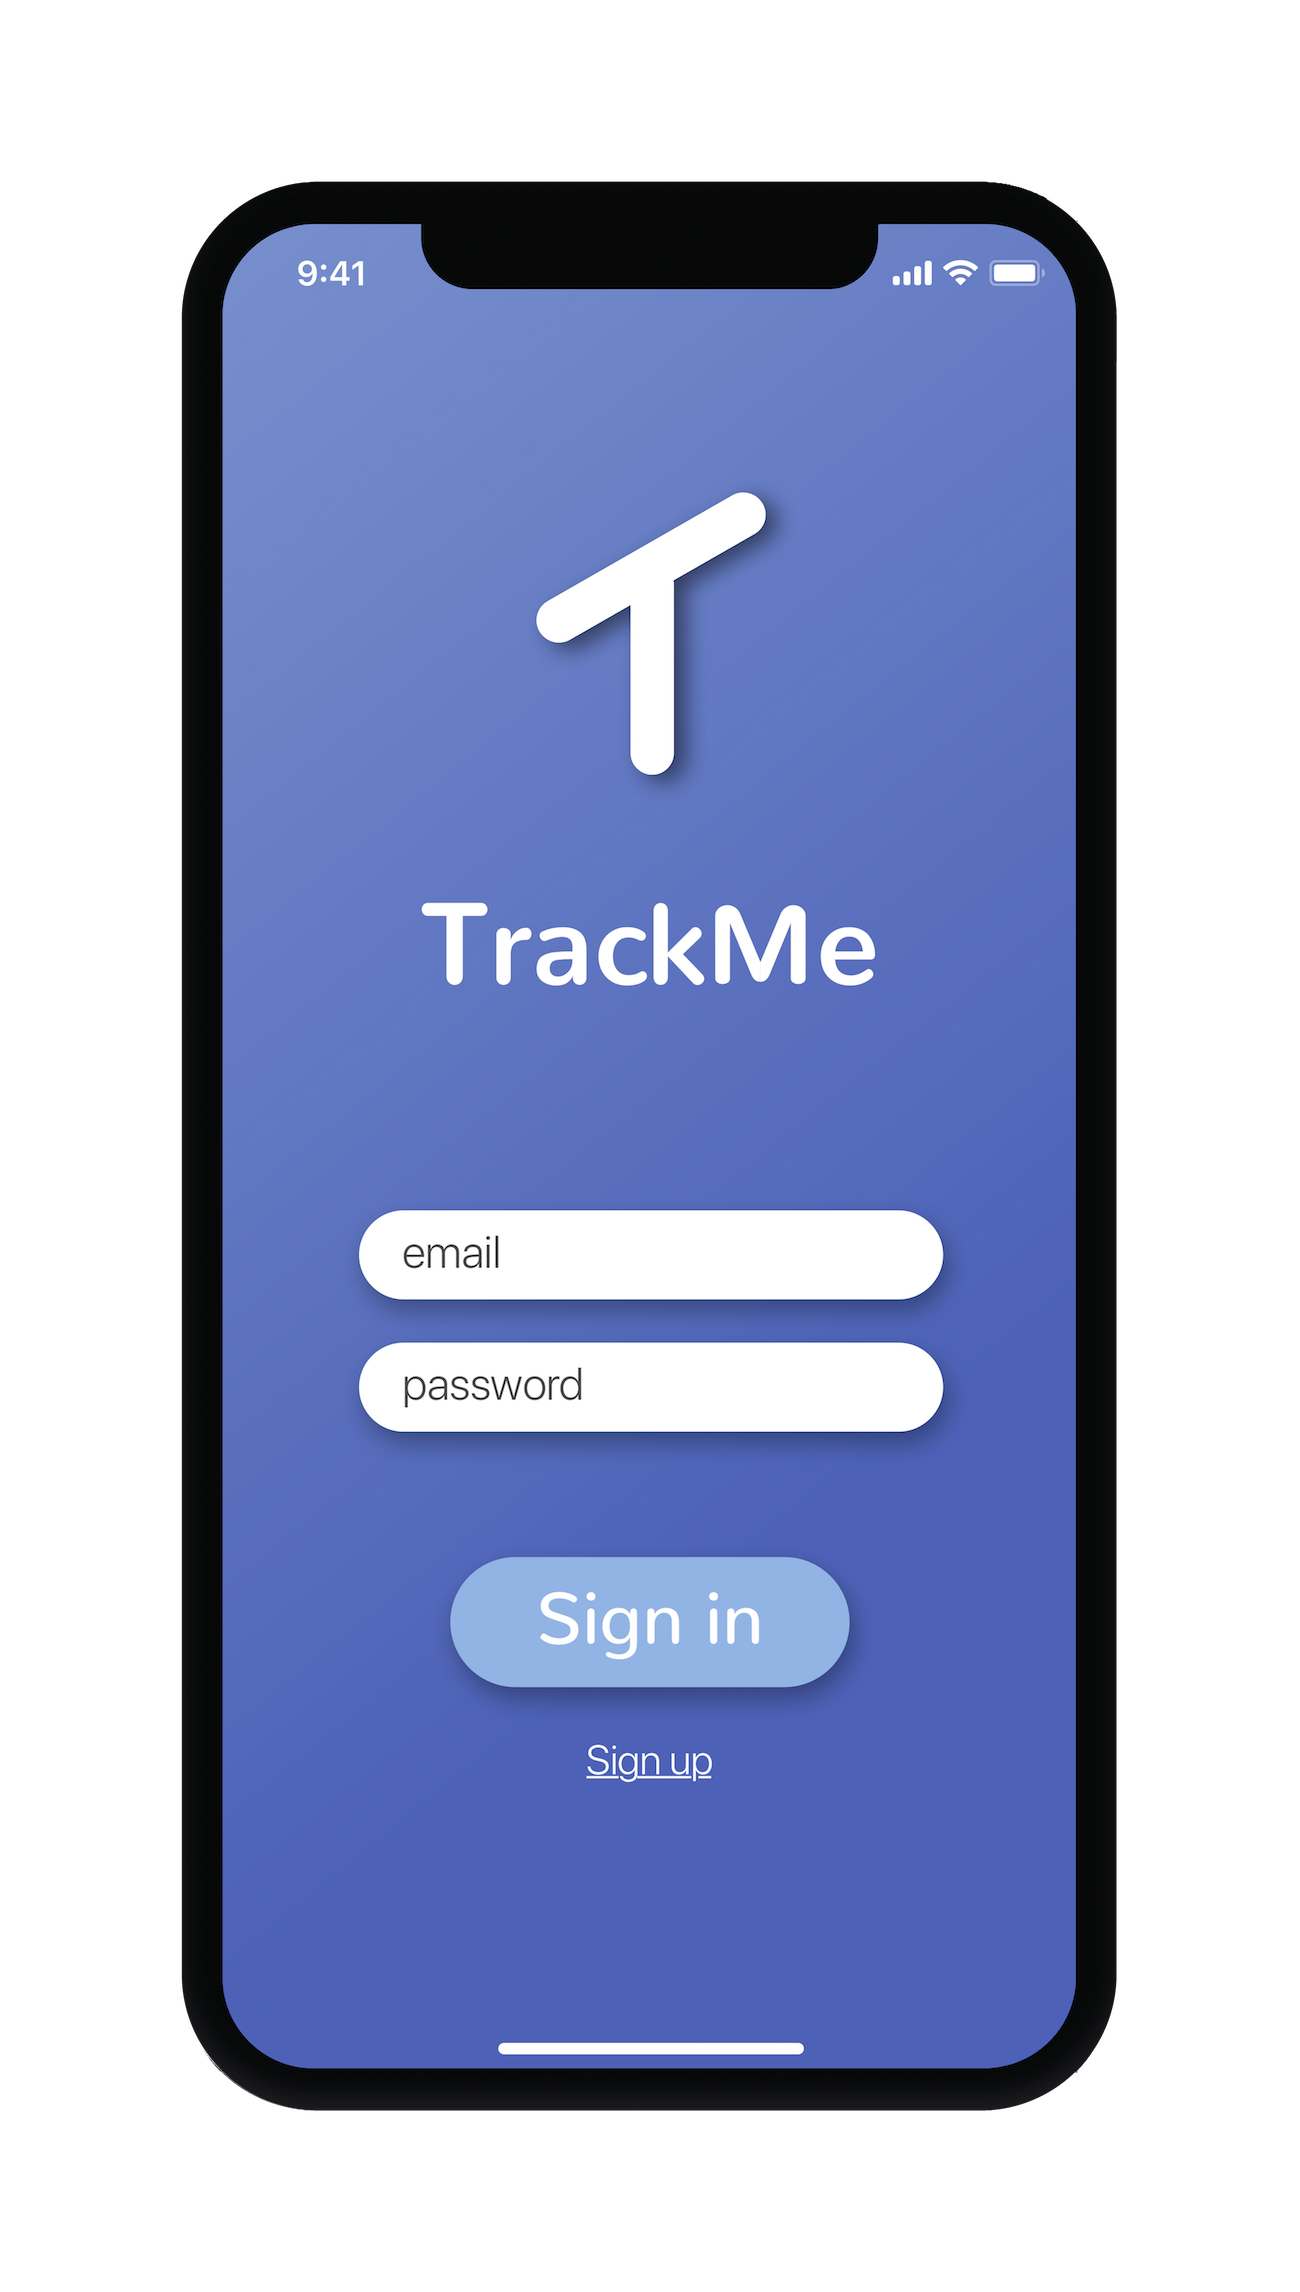
\includegraphics[width=0.4\textwidth]{./Pictures/Mockup/mobile/login.png}
    \captionsetup{skip=0pt}
    \caption{Log in}
\end{figure}



\begin{figure}[H]
\centering
\begin{subfigure}{.5\textwidth}
  \centering
  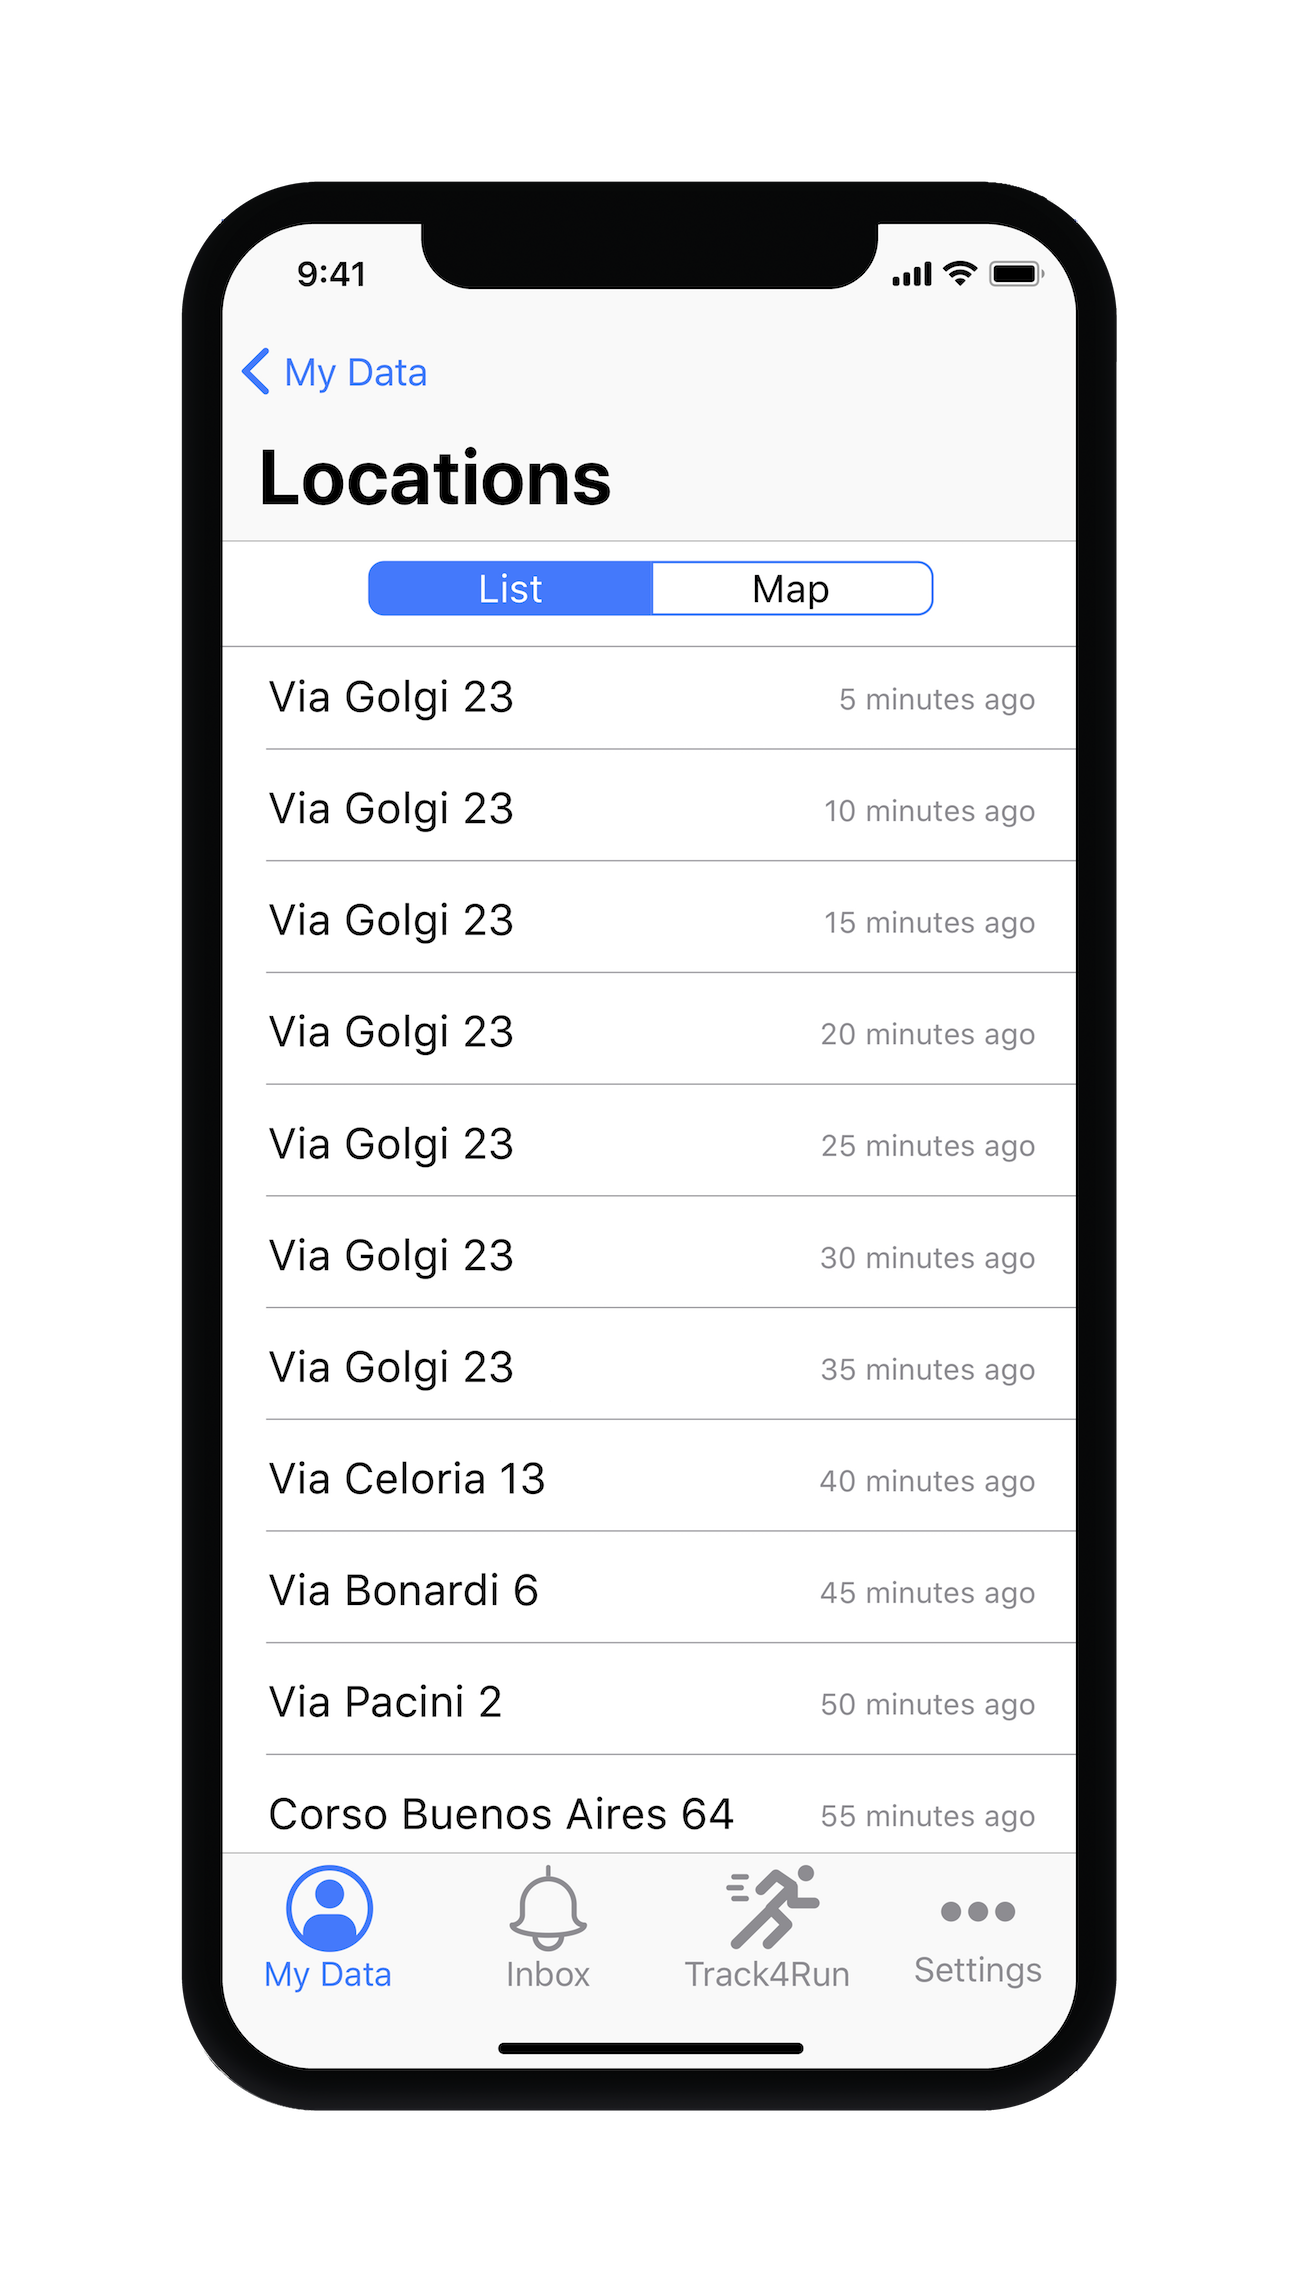
\includegraphics[width=.8\textwidth]{./Pictures/Mockup/mobile/location1.png}
  \captionsetup{skip=0pt}
  \caption{List view}
  \label{ffig:mobile-location1}
\end{subfigure}%
\begin{subfigure}{.5\textwidth}
  \centering
  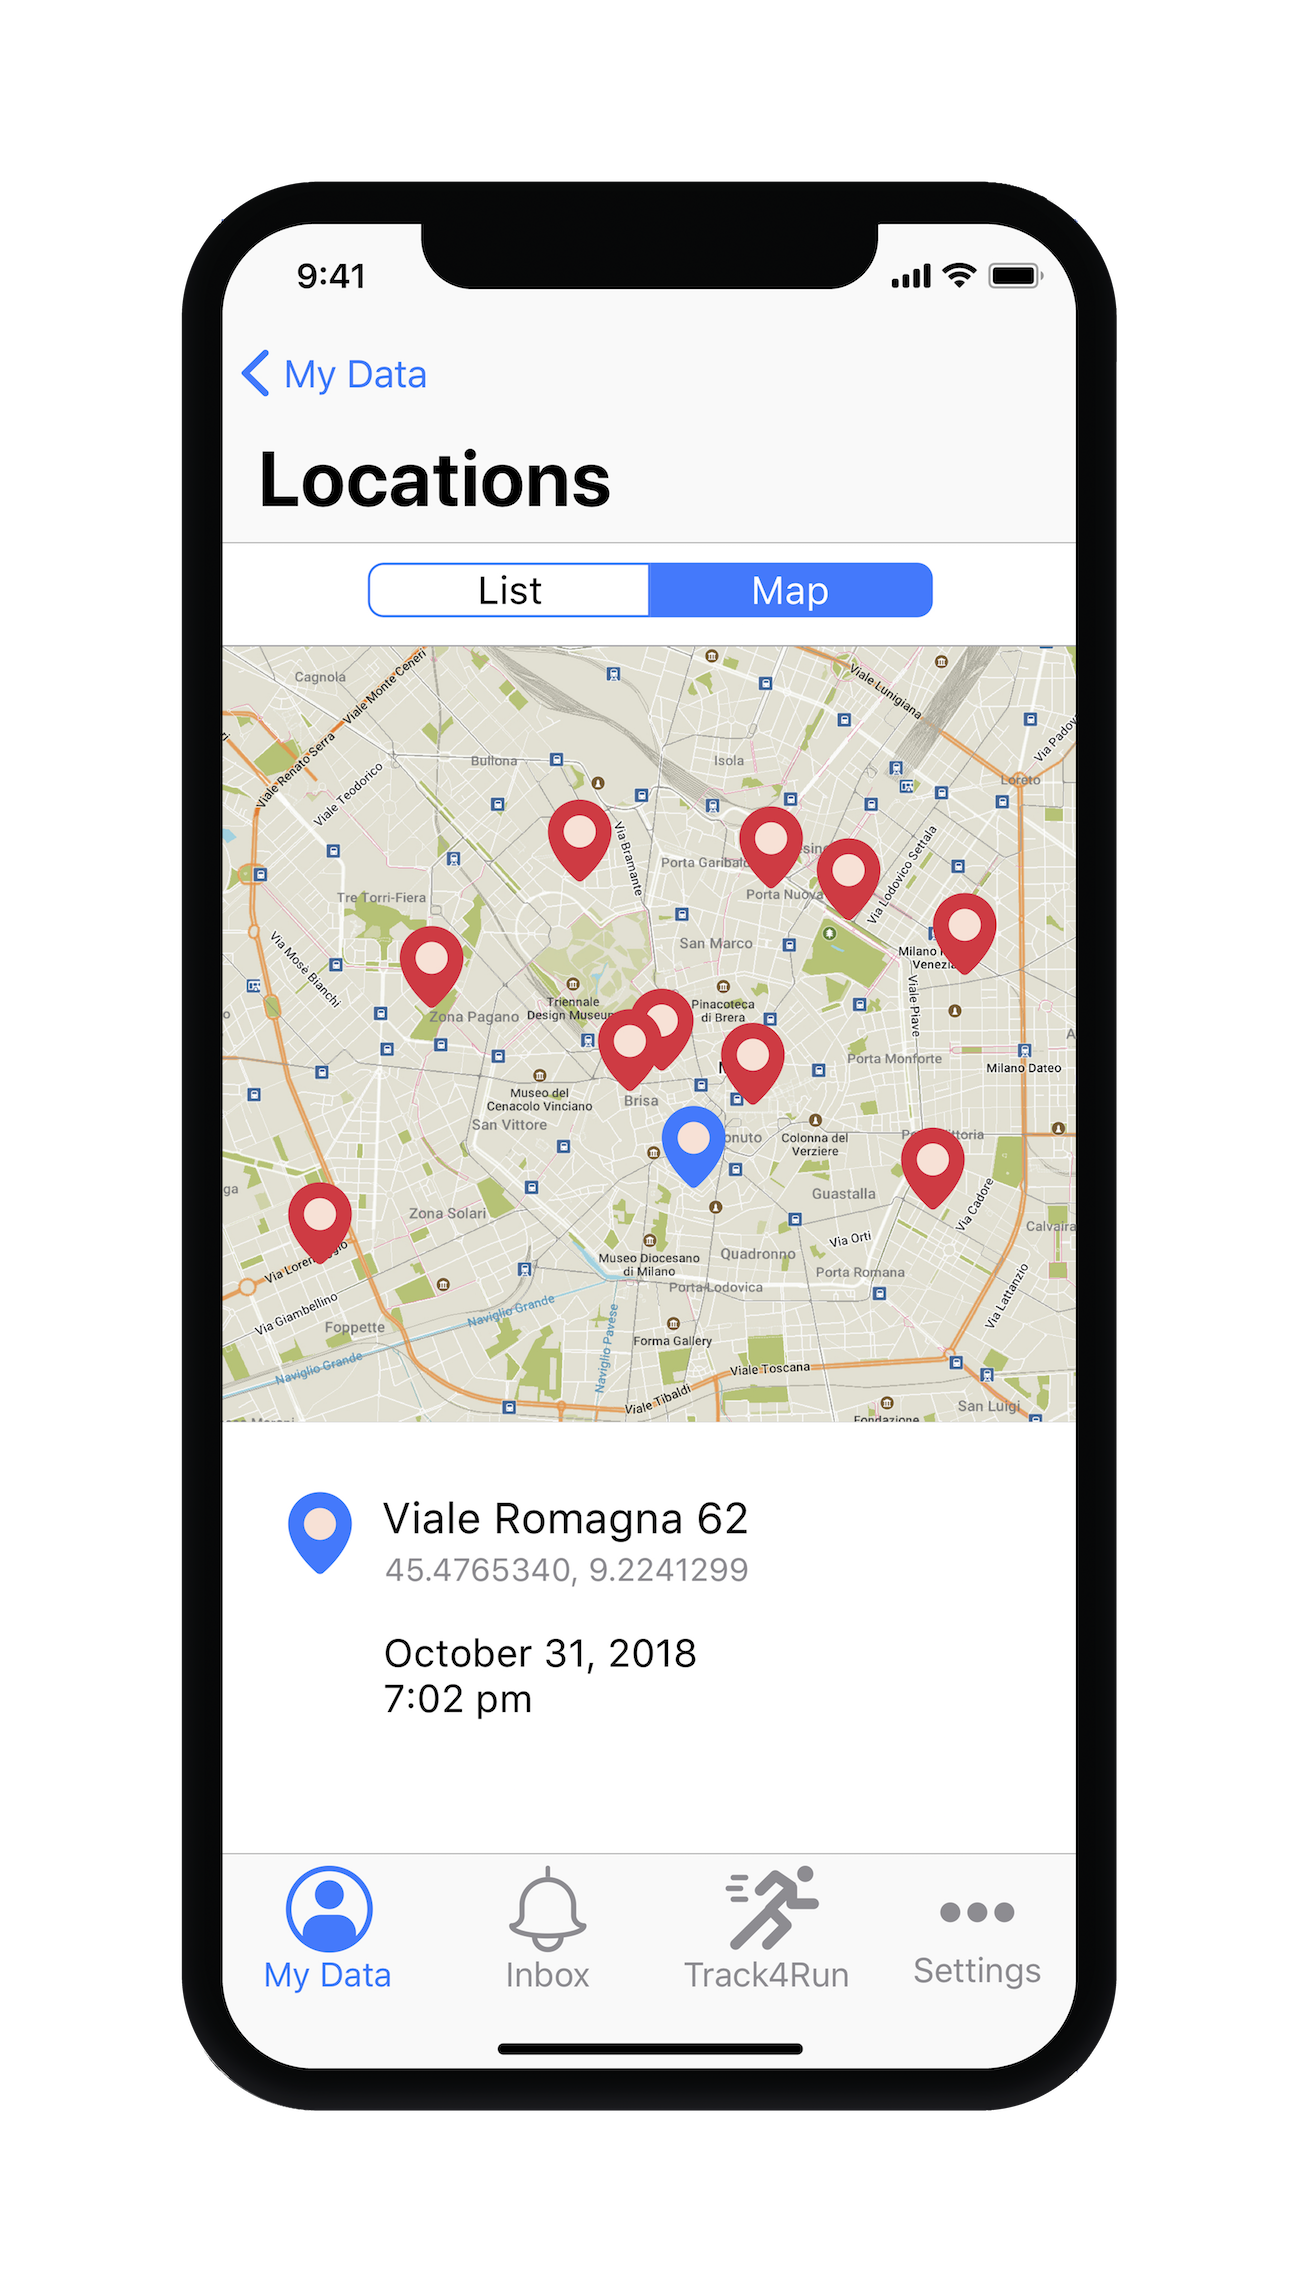
\includegraphics[width=.8\textwidth]{./Pictures/Mockup/mobile/location2.png}
  \captionsetup{skip=0pt}
  \caption{Map view}
  \label{fig:mobile-location2}
\end{subfigure}
\captionsetup{skip=8pt}
\caption{User location history}
\label{fig:test}
\end{figure}

\begin{figure}[H]
\centering
\begin{subfigure}{.5\textwidth}
  \centering
  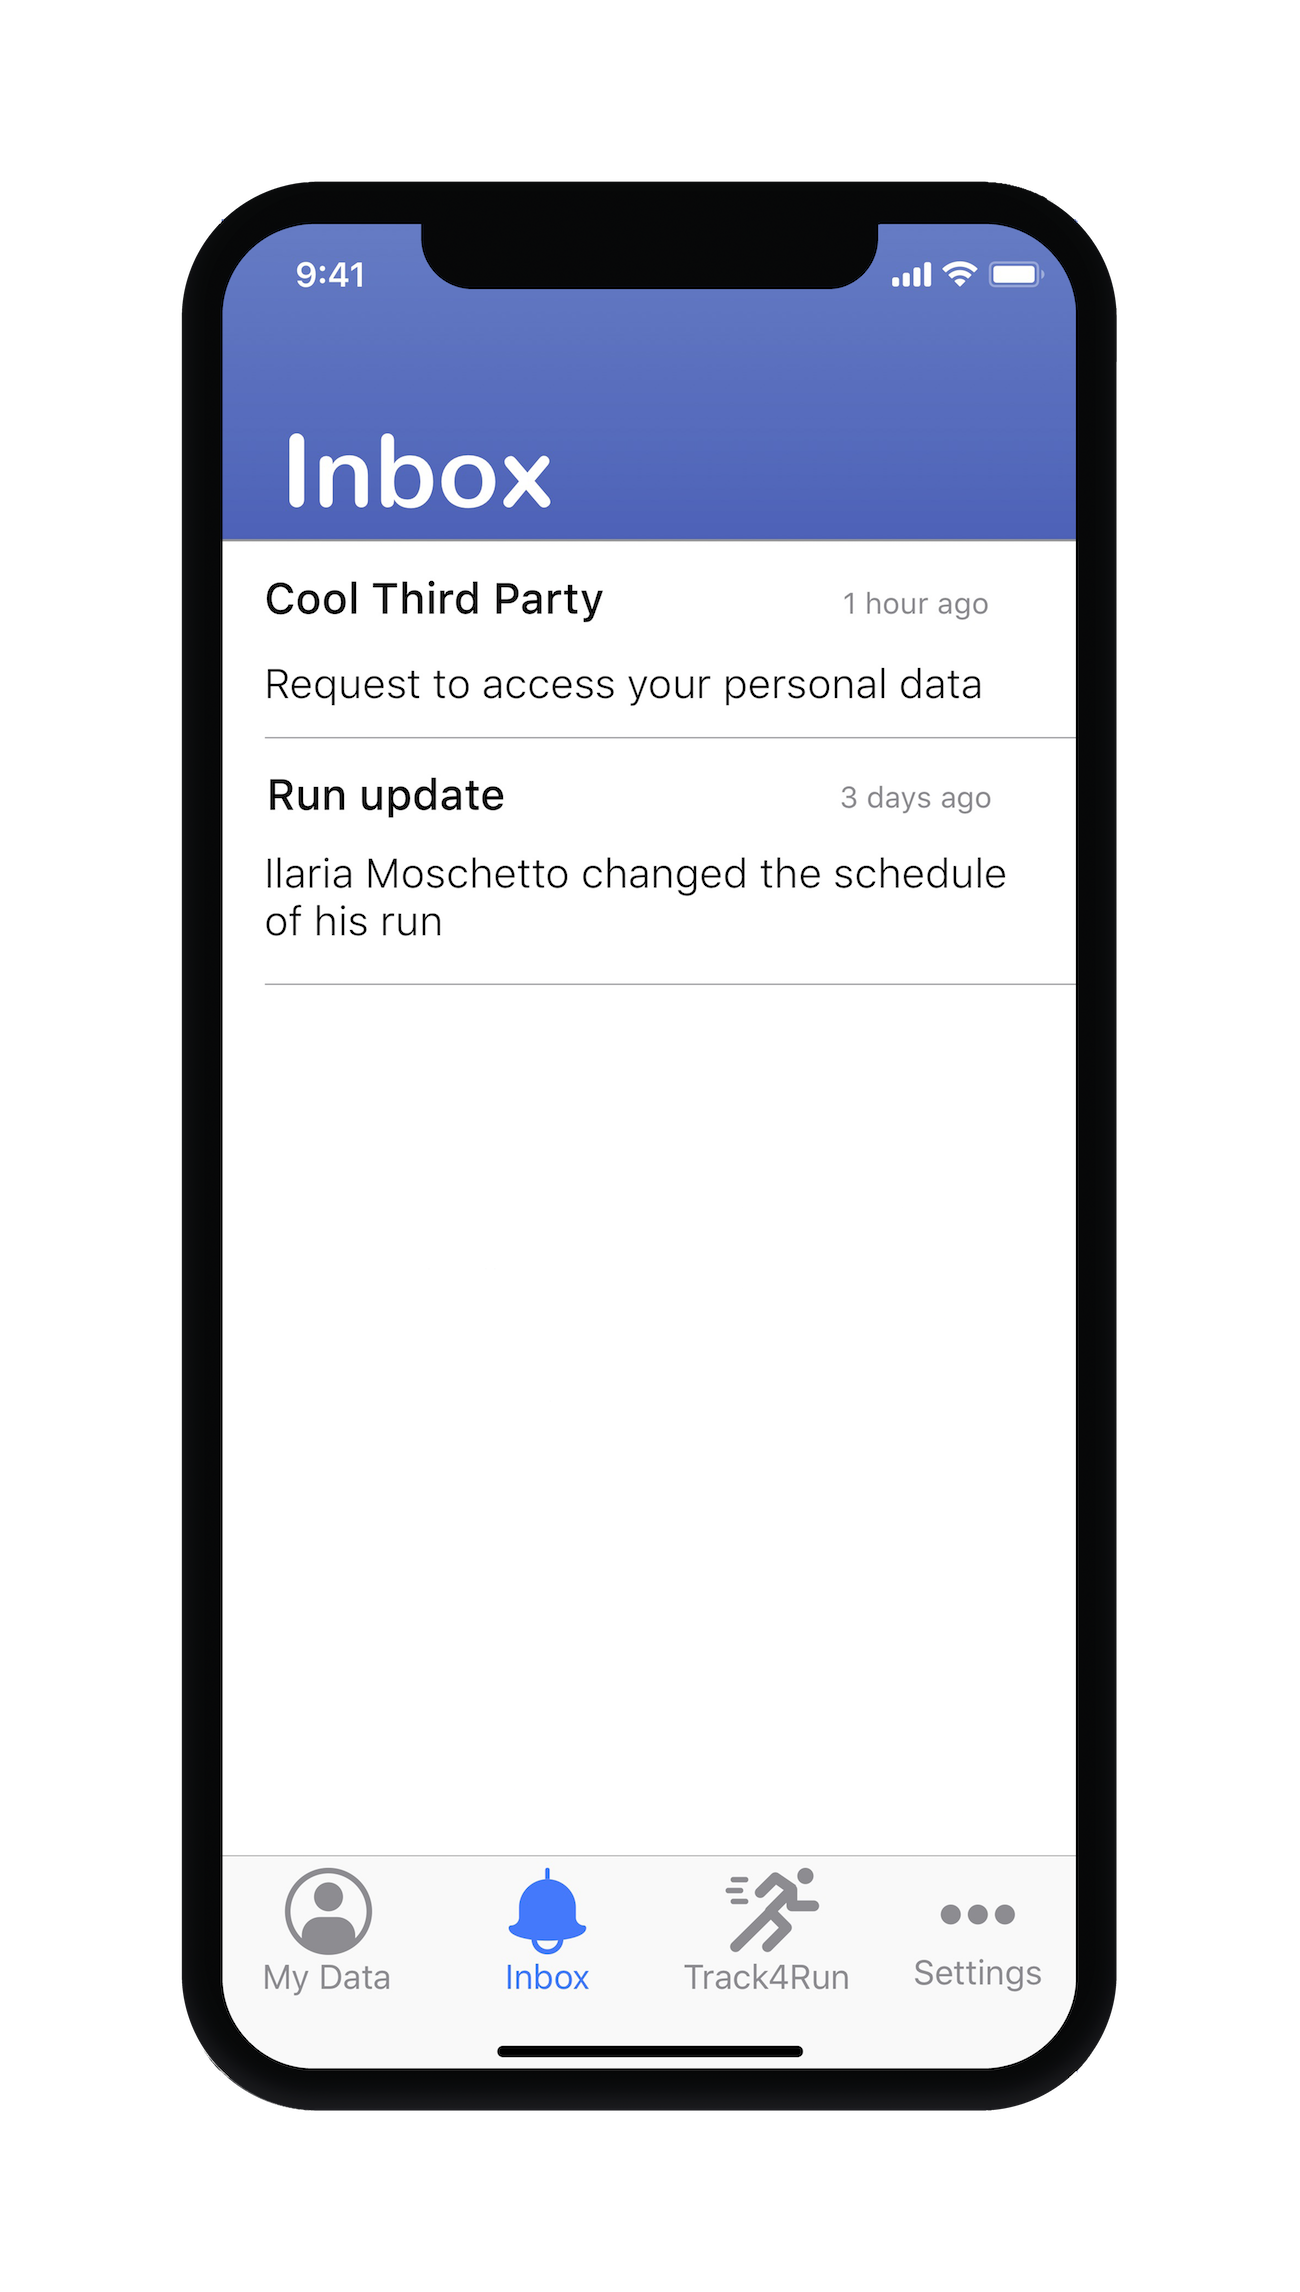
\includegraphics[width=.8\textwidth]{./Pictures/Mockup/mobile/inbox.png}
  \captionsetup{skip=0pt}
  \caption{Received requests view}
  \label{ffig:mobile-inbox}
\end{subfigure}%
\begin{subfigure}{.5\textwidth}
  \centering
  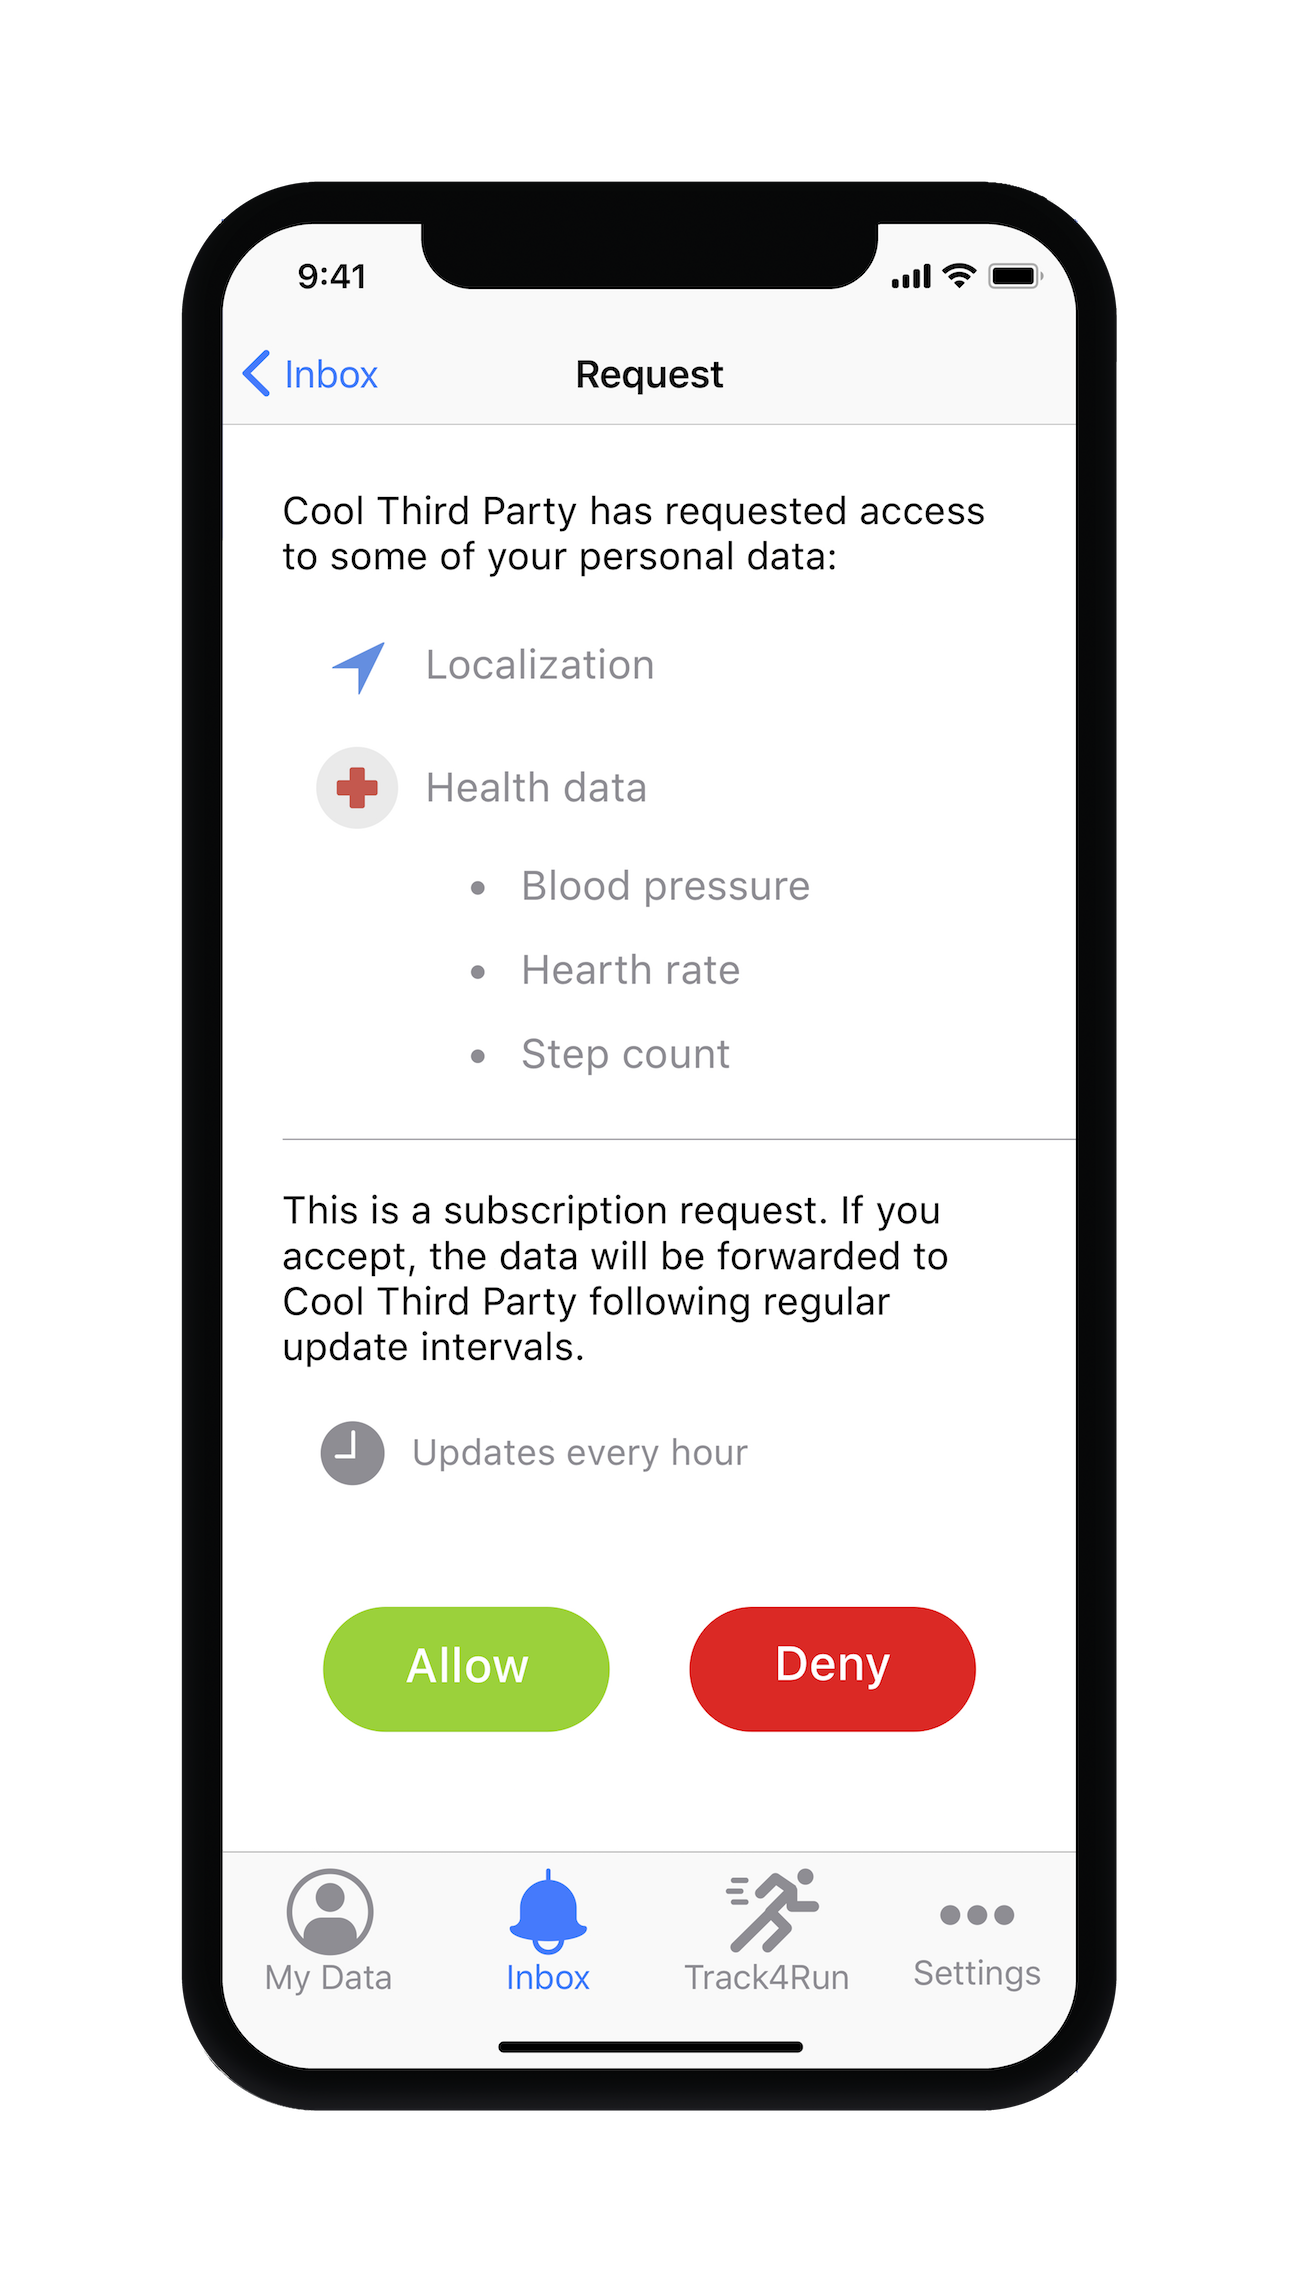
\includegraphics[width=.8\textwidth]{./Pictures/Mockup/mobile/request_received.png}
  \captionsetup{skip=0pt}
  \caption{Request reply view}
  \label{fig:mobile-request}
\end{subfigure}
\captionsetup{labelformat=empty}
\label{fig:test}
\end{figure}

\begin{figure}[H]
	\centering
	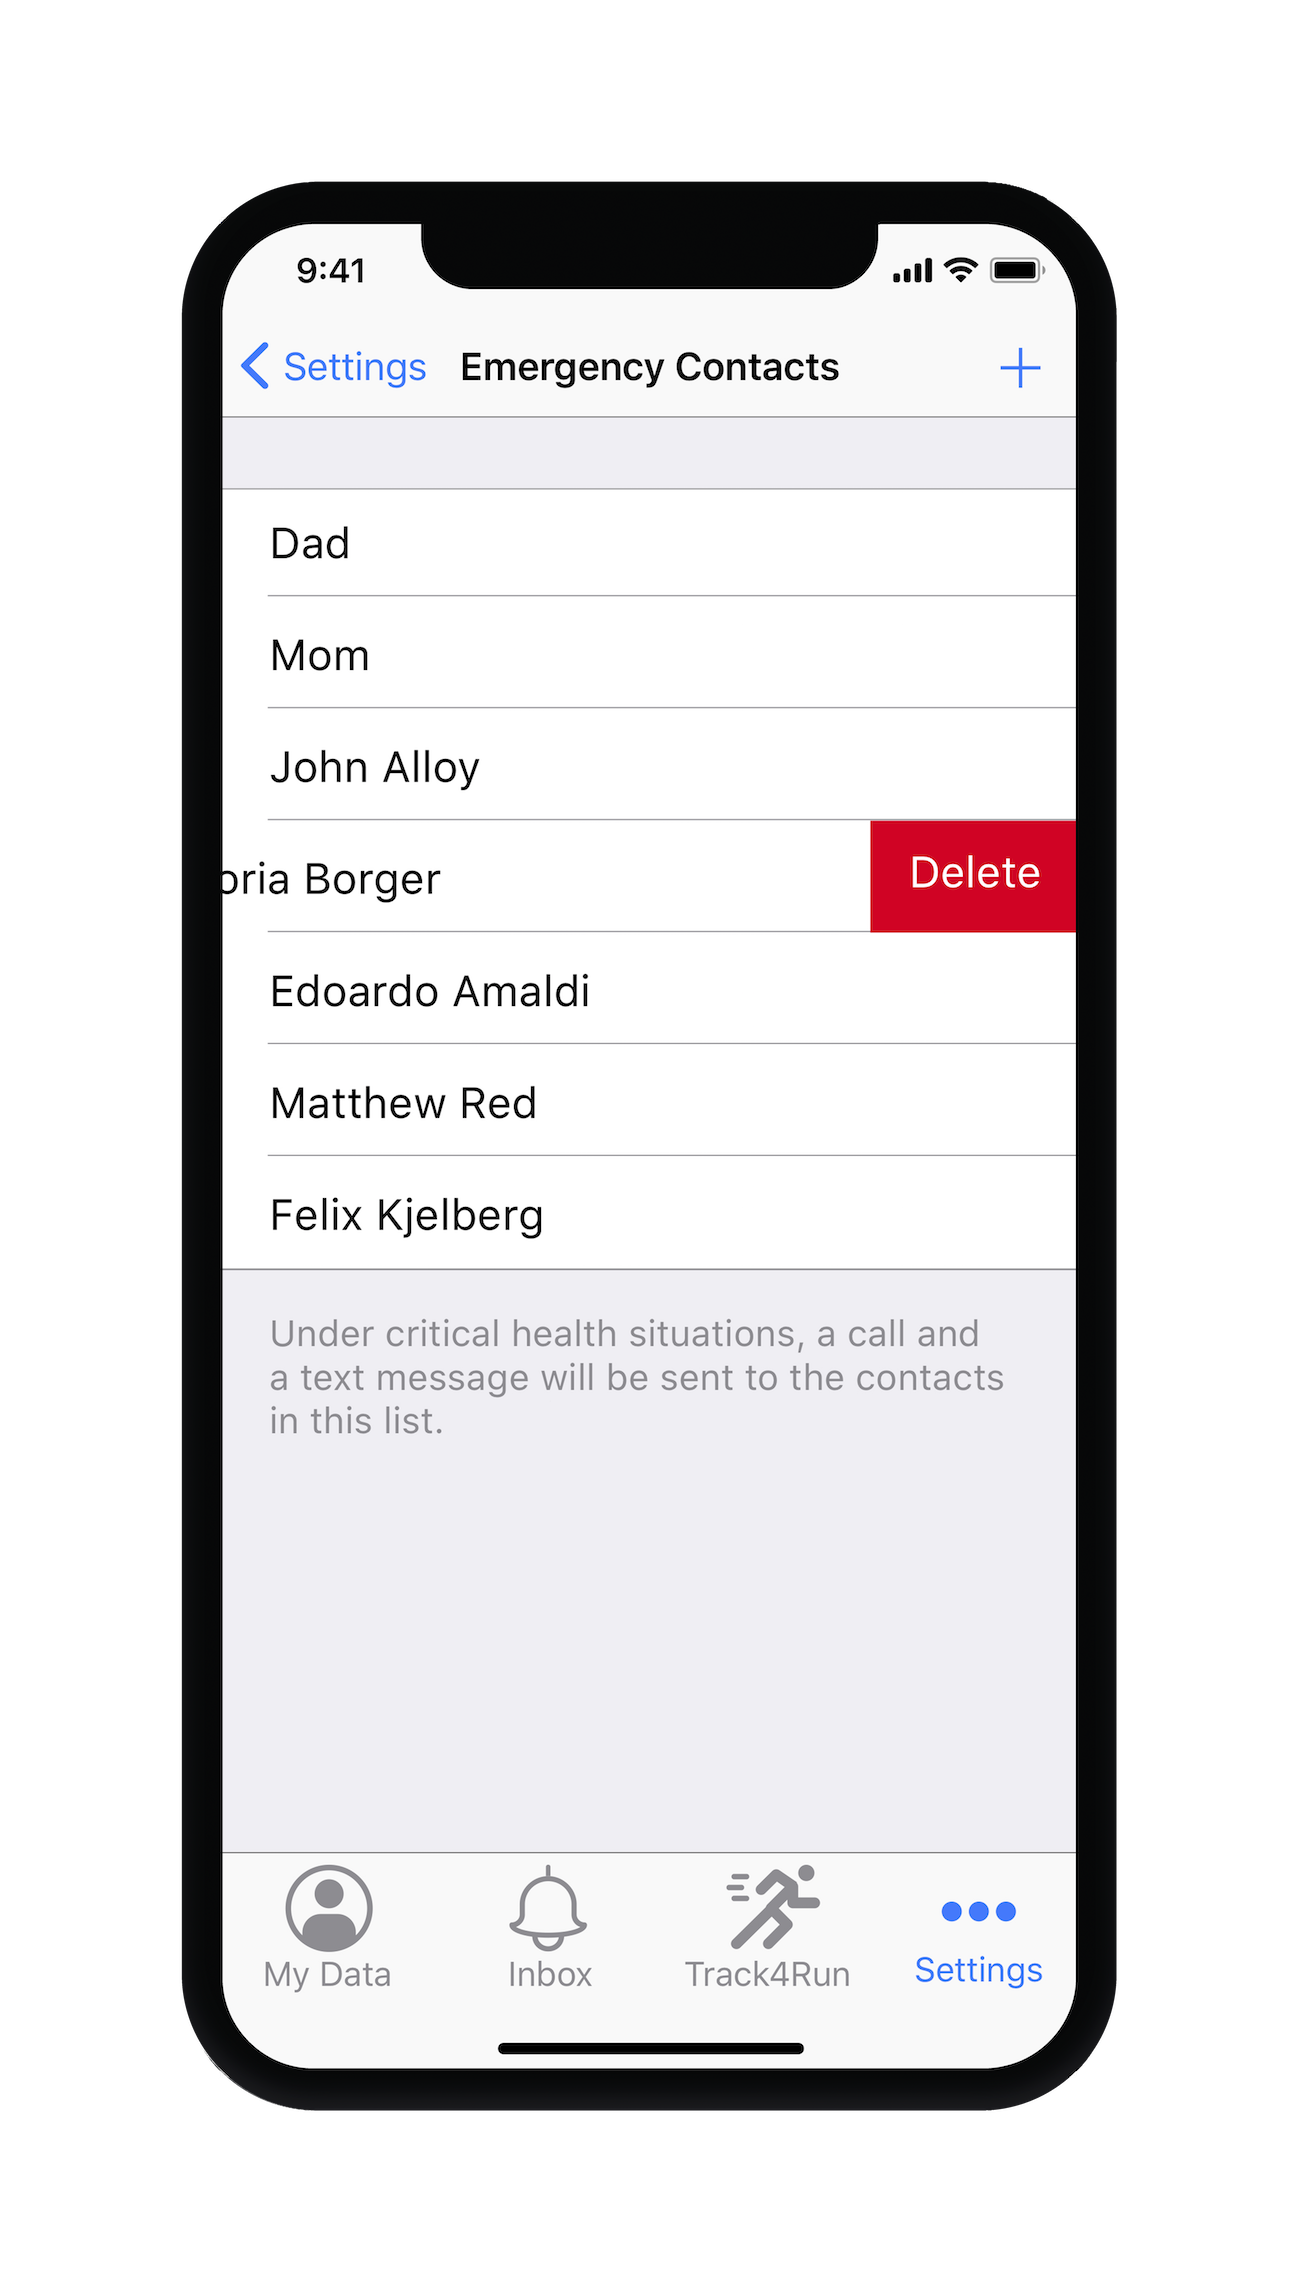
\includegraphics[width=0.4\textwidth]{./Pictures/Mockup/mobile/emergency_contacts.png}
	\captionsetup{skip=0pt}
	\caption{List of contacts to be informed in case of emergency}
\end{figure}


\begin{figure}[H]
	\centering
	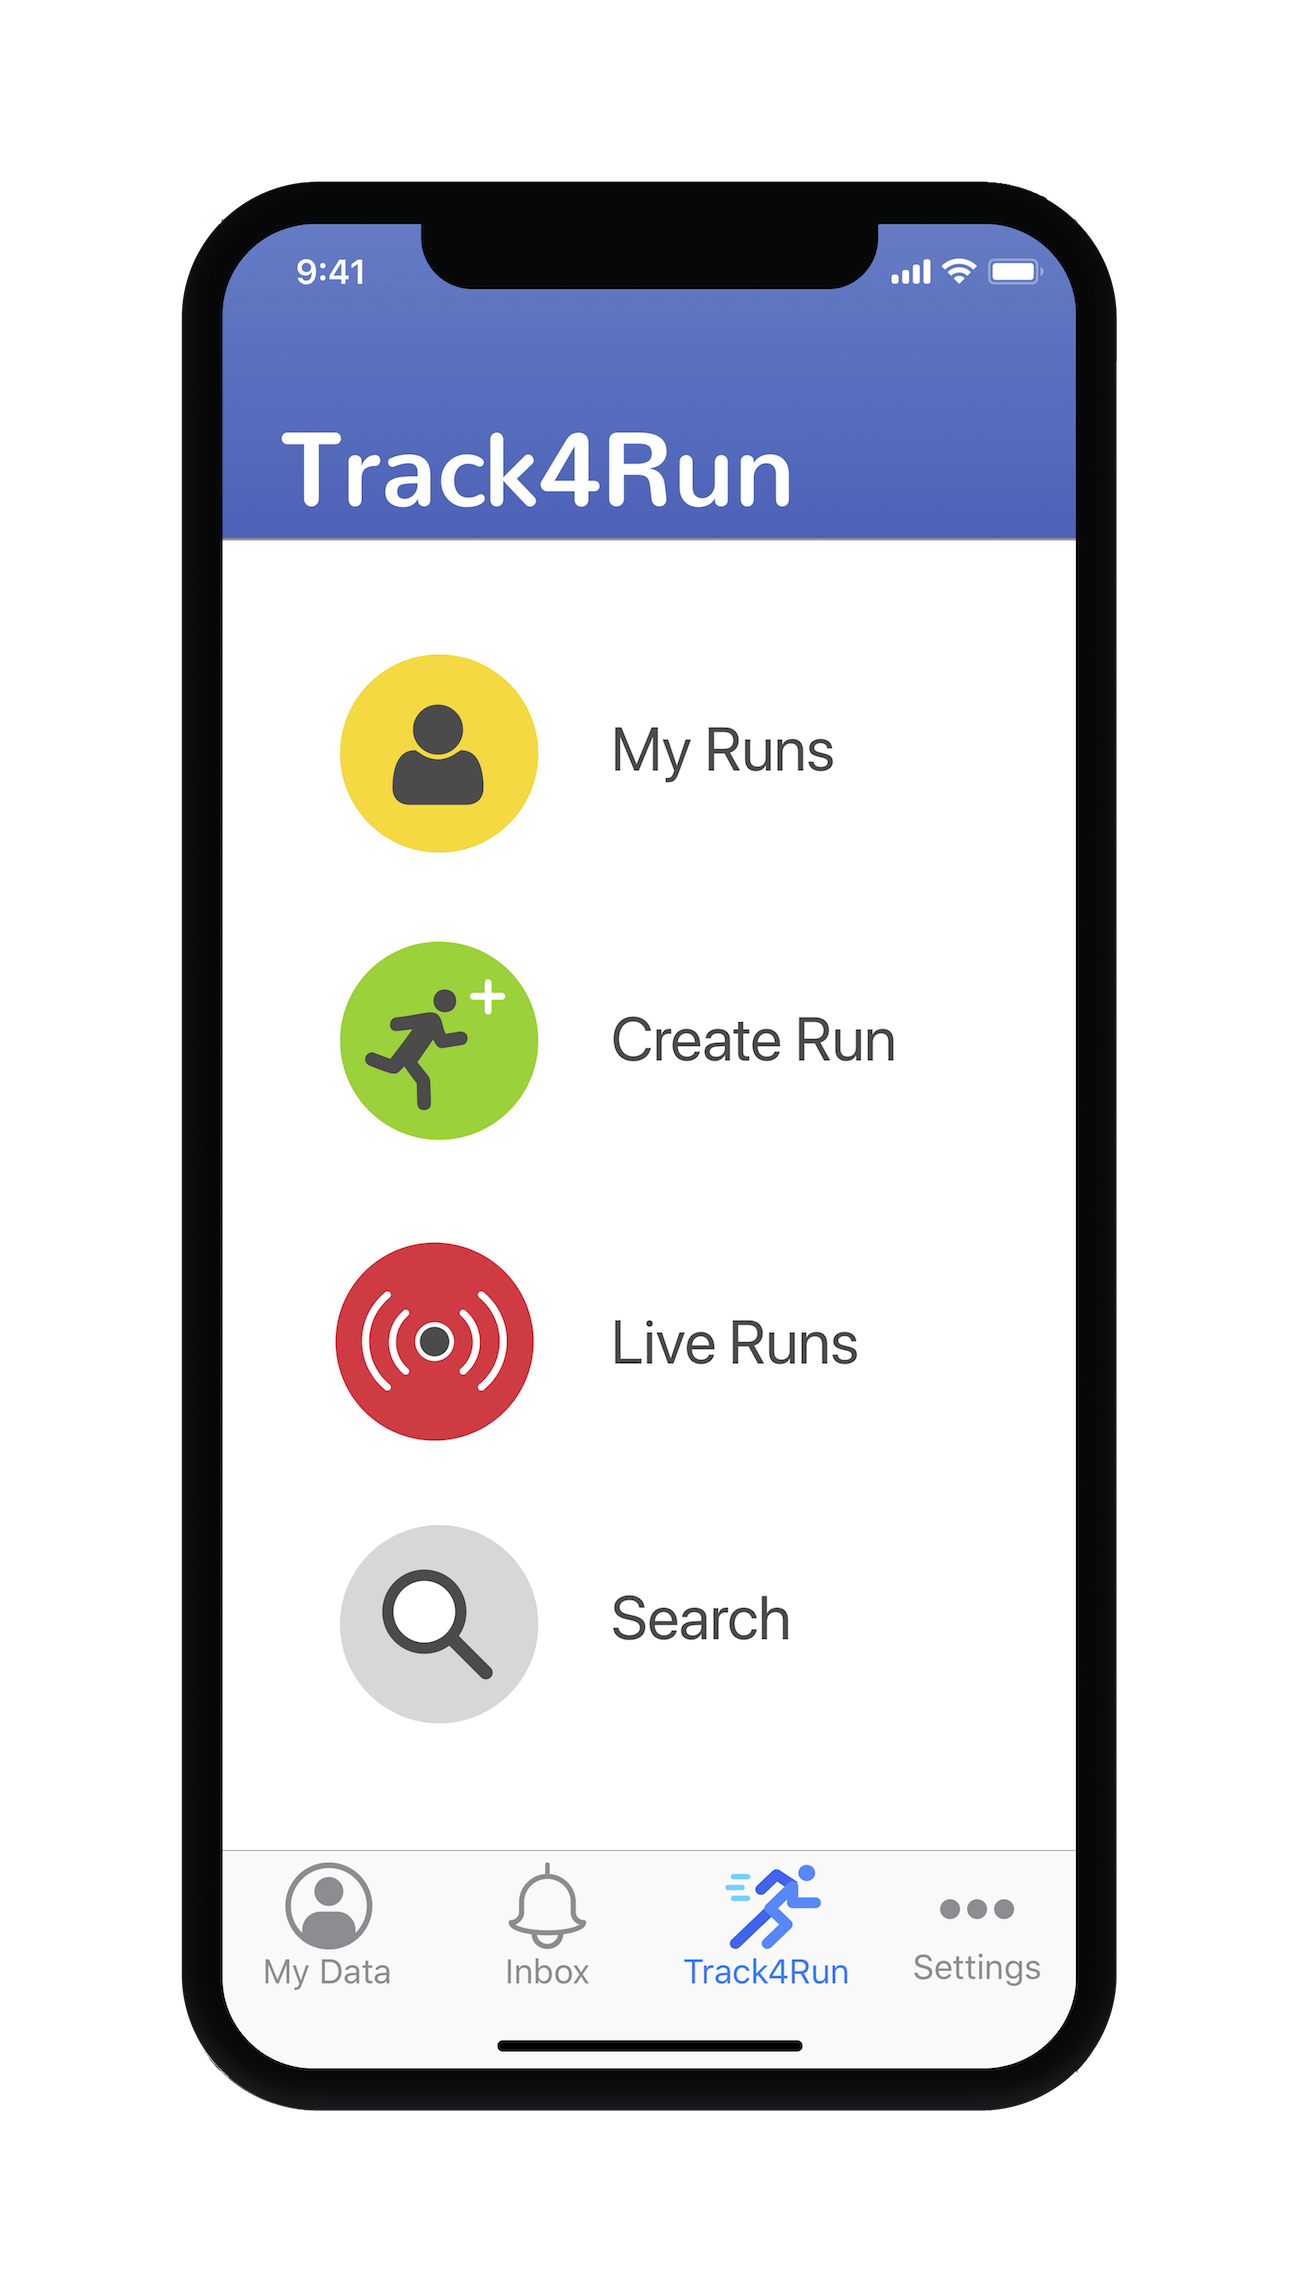
\includegraphics[width=0.4\textwidth]{./Pictures/Mockup/mobile/track4run.png}
	\captionsetup{skip=0pt}
	\caption{Track4Run main view}
\end{figure}

\begin{figure}[H]
	\centering
	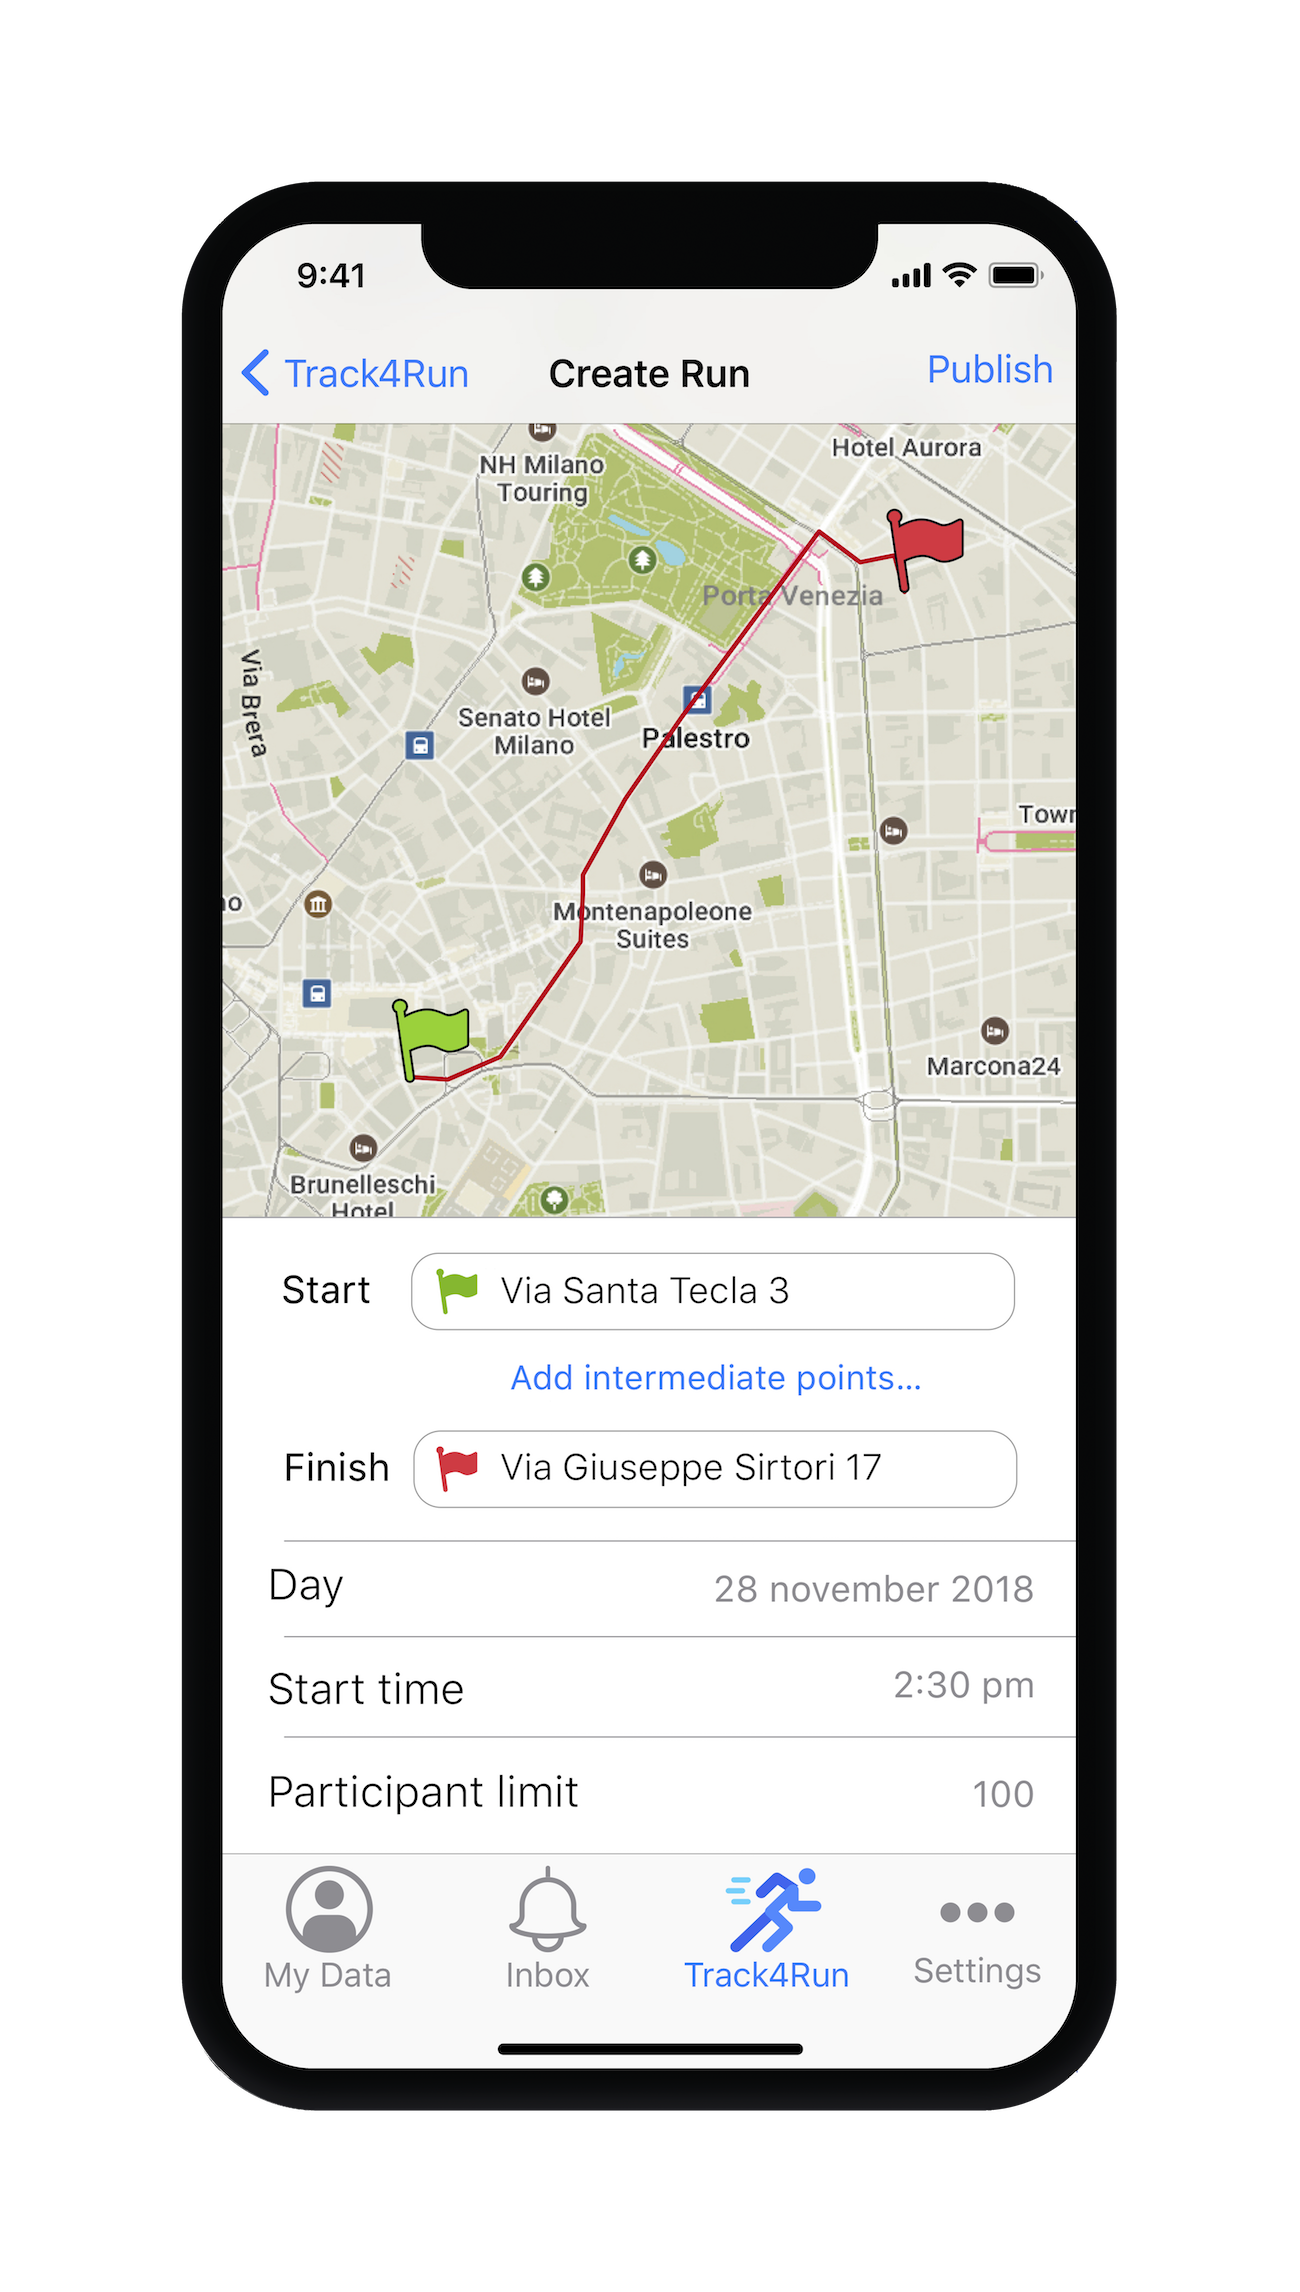
\includegraphics[width=0.4\textwidth]{./Pictures/Mockup/mobile/create_run.png}
	\captionsetup{skip=0pt}
	\caption{Create run view}
\end{figure}

\begin{figure}[H]
	\centering
	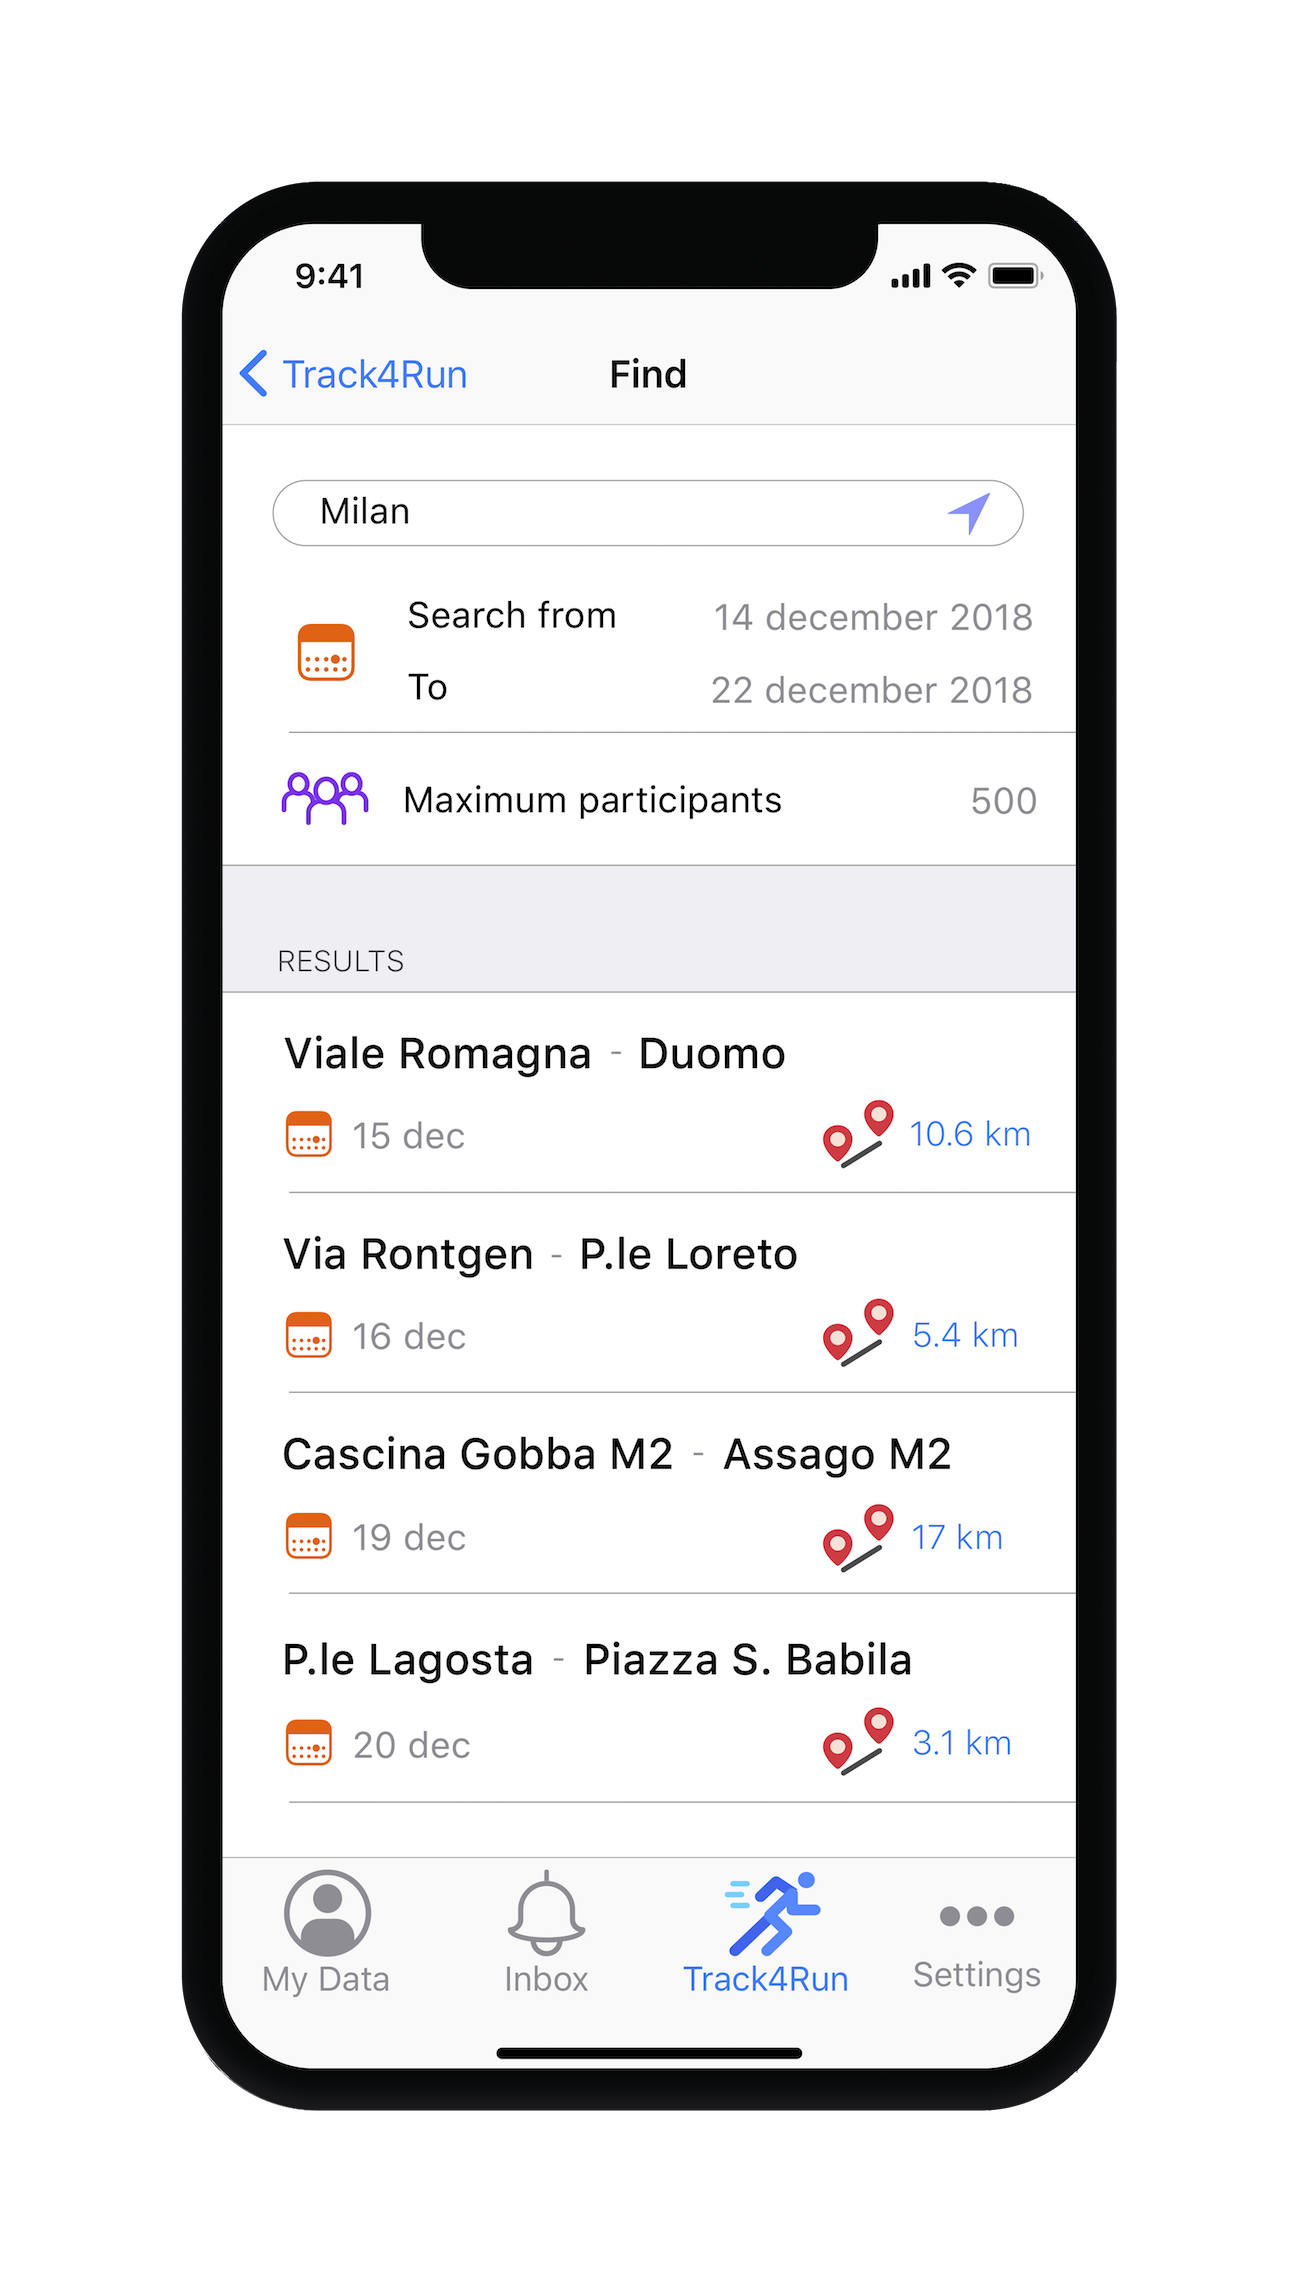
\includegraphics[width=0.4\textwidth]{./Pictures/Mockup/mobile/search_run.png}
	\captionsetup{skip=0pt}
	\caption{Search run view}
\end{figure}

\begin{figure}[H]
	\centering
	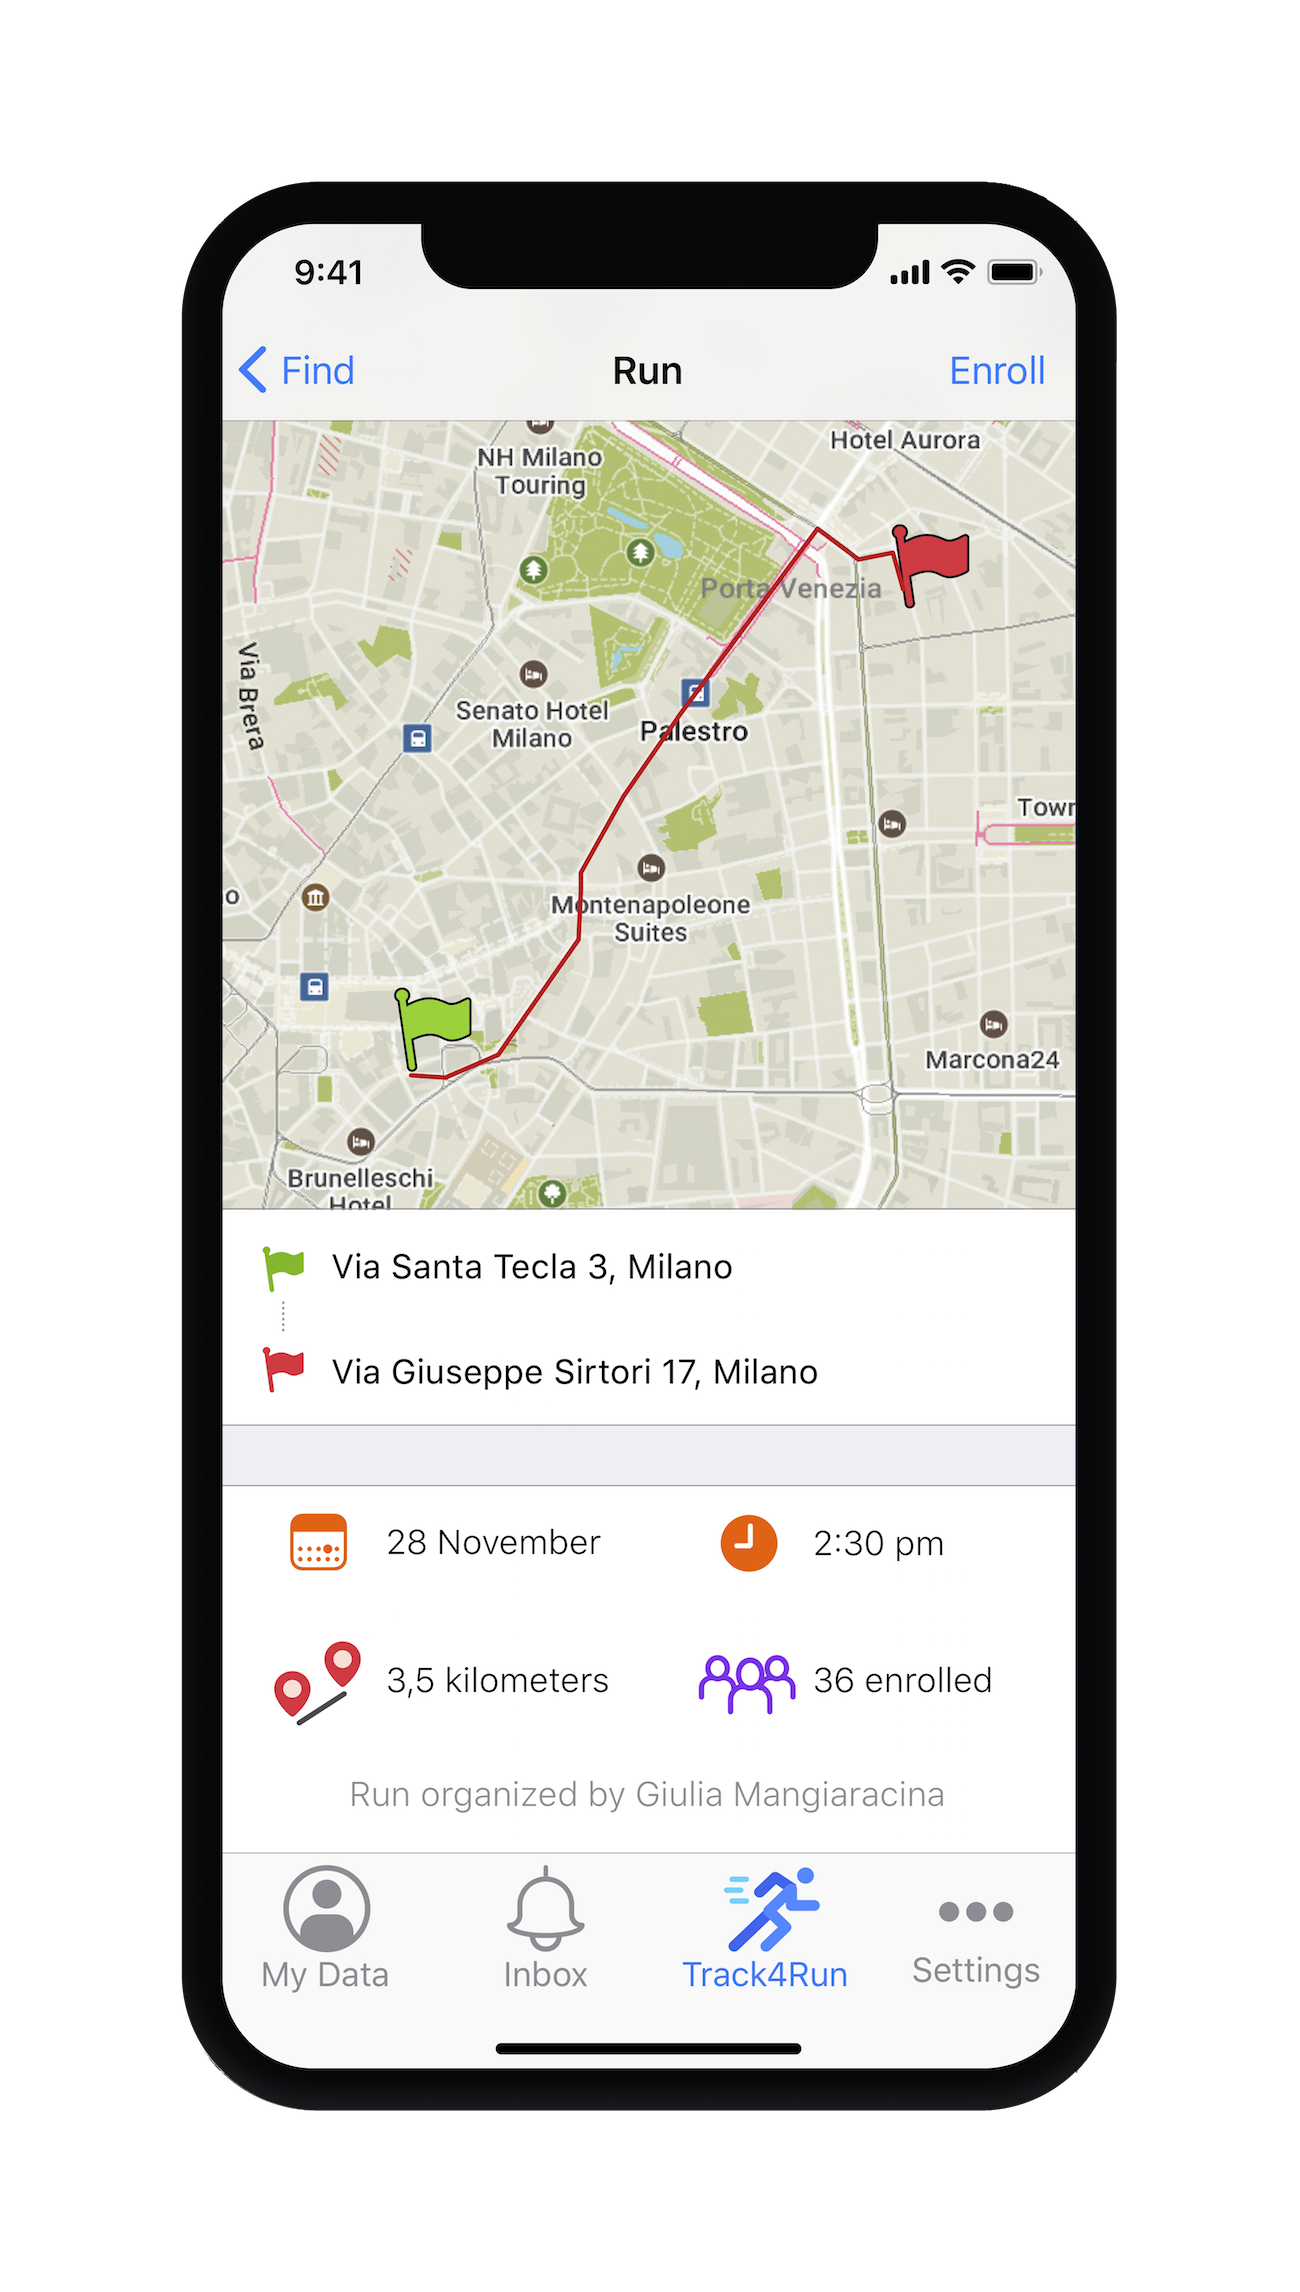
\includegraphics[width=0.4\textwidth]{./Pictures/Mockup/mobile/view_run.png}
	\captionsetup{skip=0pt}
	\caption{Run details view}
\end{figure}

\begin{figure}[H]
	\centering
	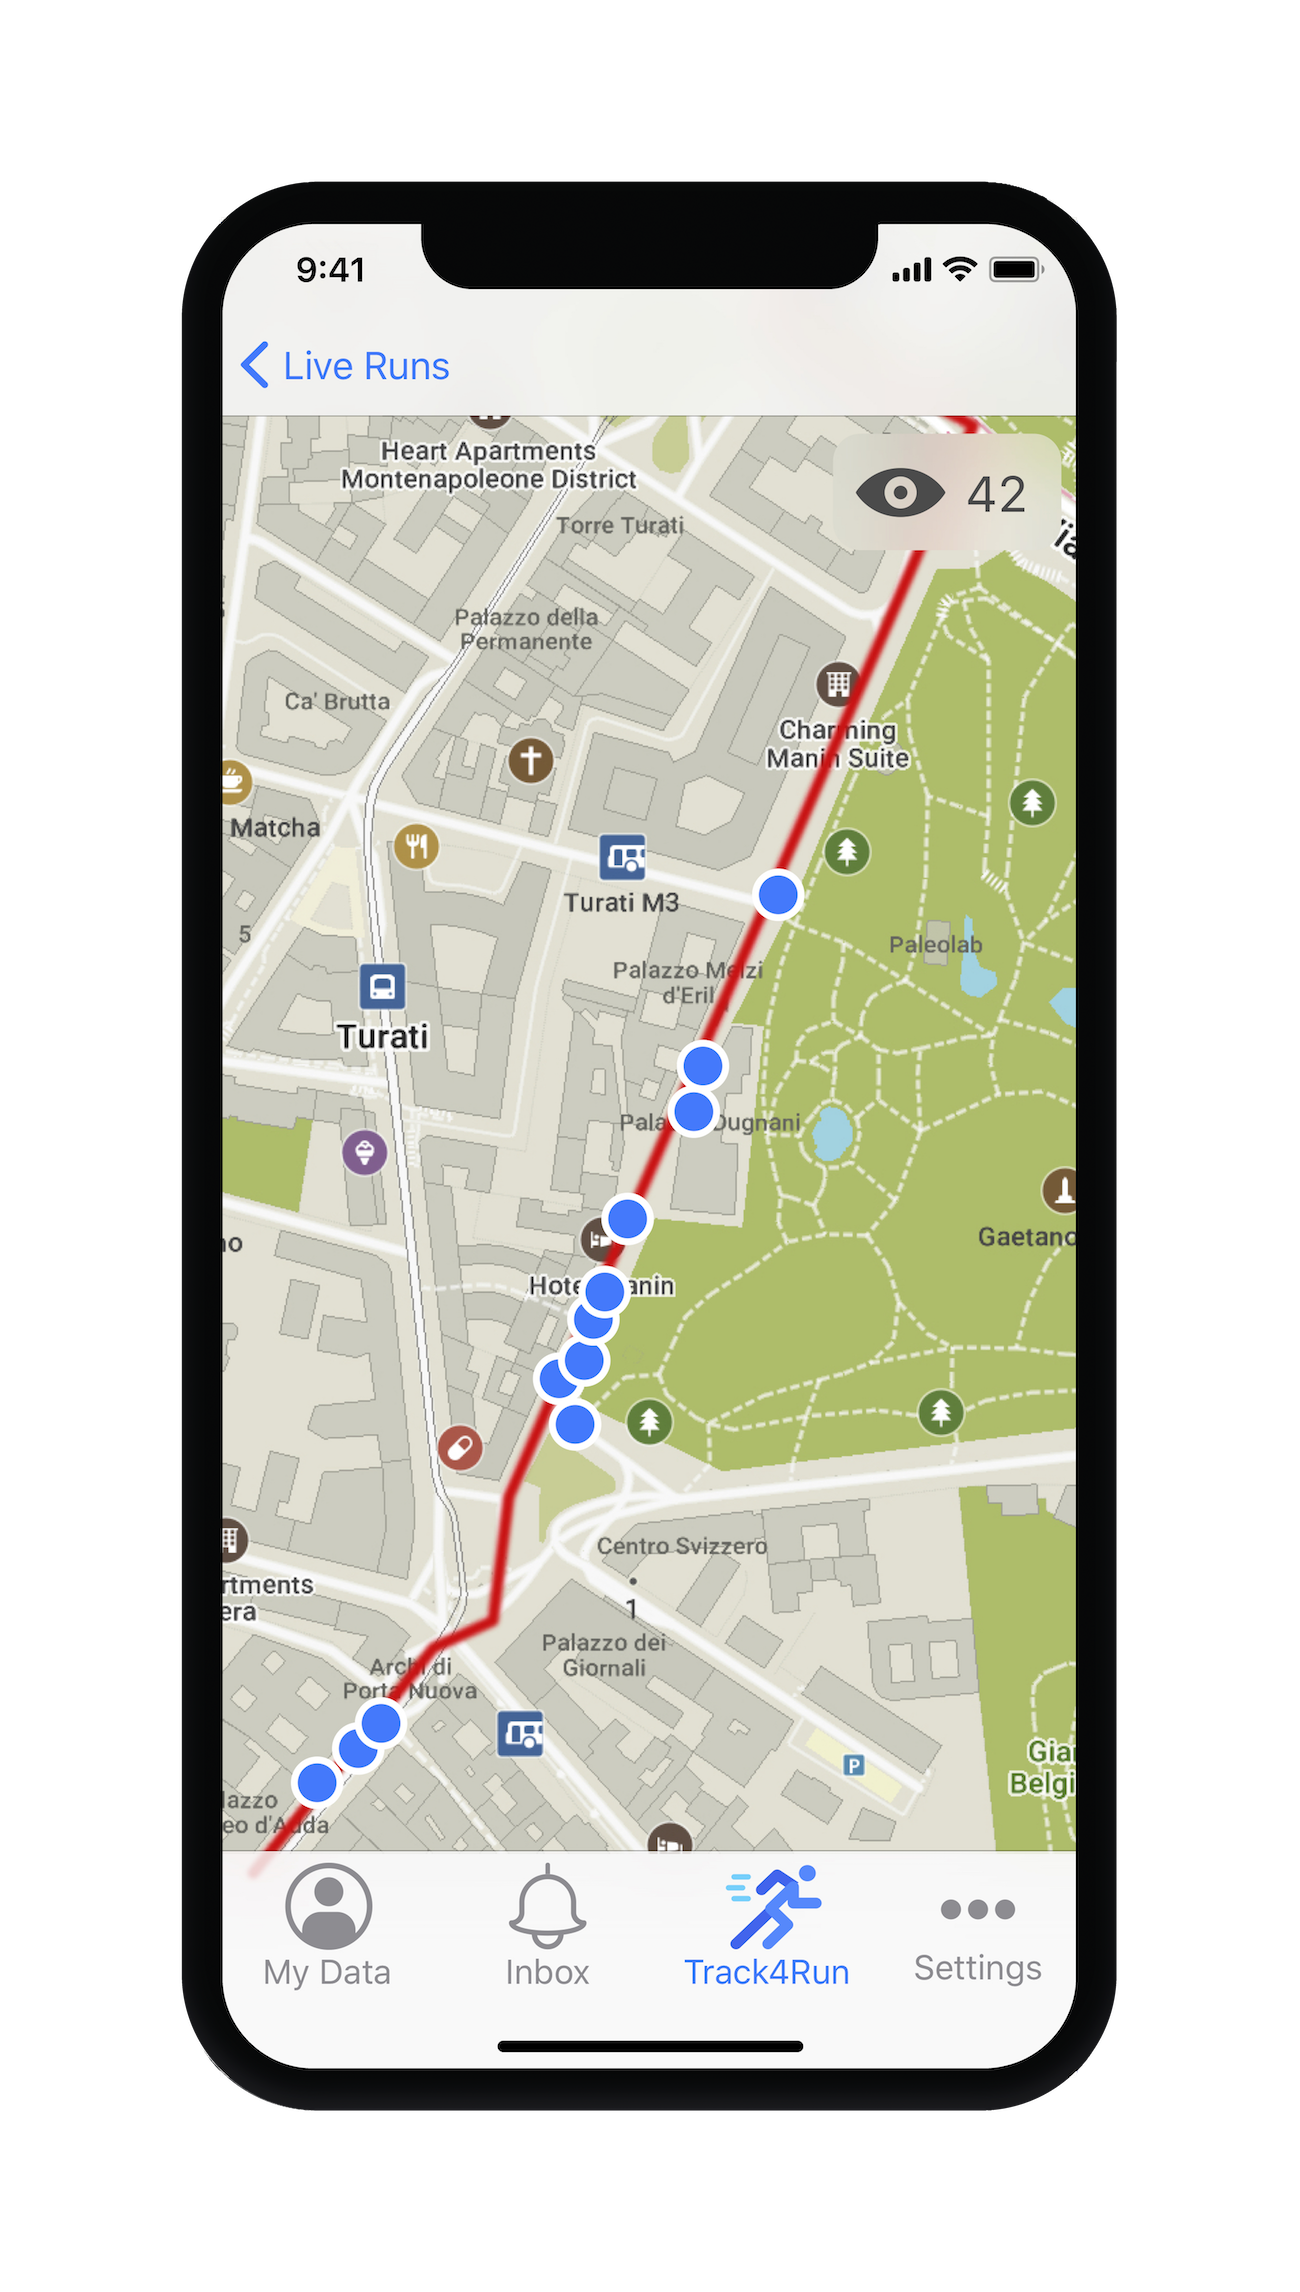
\includegraphics[width=0.4\textwidth]{./Pictures/Mockup/mobile/visitor_view.png}
	\captionsetup{skip=0pt}
	\caption{Live run view}
\end{figure}



























